%-------------------------------------------------------------------------------
% yum_menu
%-------------------------------------------------------------------------------
%
% \file        yum_menu.tex
% \library     Documents
% \author      Chris Ahlstrom
% \date        2015-05-11
% \update      2017-09-03
% \version     $Revision$
% \license     $XPC_GPL_LICENSE$
%
%     Provides the Menu section of yoshimi-user-manual.tex.
%
%-------------------------------------------------------------------------------

\section{Menu}
\label{sec:menu}

   At last, we're now ready to describe the user-interface of \textsl{Yoshimi}!
   The \textsl{Yoshimi} menu, as seen at the top of
   \figureref{fig:yoshimi_main_screen},
   is fairly simple, but it is important to understand the
   structure of the menu entries.

\subsection{Menu / Yoshimi}
\label{subsec:menu_yoshimi}

   The \textsl{Yoshimi}
   menu entry contains the sub-items shown in
   \figureref{fig:yoshimi_menu_items}.
   The next few sub-sections discuss the sub-items in the 
   \textsl{Yoshimi} sub-menu.
   (Note that, in \textsl{ZynAddSubFX}, this menu is called the
   \textsl{File} menu.)

\begin{figure}[H]
   \centering 
%  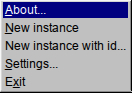
\includegraphics[scale=0.75]{menu/yoshimi-menu-yoshimi.jpg}
%  \includegraphics[scale=1.0]{1.4.0/yoshimi-menu-yoshimi.png}
%  \includegraphics[scale=1.0]{1.4.1/yoshimi-menu-yoshimi.png}
%  \includegraphics[scale=1.0]{1.5.0/yoshimi-menu-yoshimi.png}
   \includegraphics[scale=1.0]{1.5.3/yoshimi-menu-yoshimi.png}
   \caption{Yoshimi Menu Items}
   \label{fig:yoshimi_menu_items}
\end{figure}

   The items it contains are:

   \begin{enumber}
      \item \textbf{About...}
      \item \textbf{New instance}
      \item \textbf{Settings...}
      \item \textbf{MIDI Learn...}
      \item \textbf{Exit}
   \end{enumber}

   \textbf{New:}
   \index{new!vectors}
   The \textbf{Vectors} menu entry of version 1.4.0 has been moved to its own
   button in version 1.4.1, as can be seen in the figure.  See
   \sectionref{subsec:vector_dialogs}, which presents this dialog and
   describes it.

   \textbf{New:}
   \index{new!MIDI Learn}
   \textsl{MIDI Learn} is a new feature of \textsl{Yoshimi}, and is described
   below.

% Now fixed!
%
%  \textbf{Bug:}
%  \index{bugs!menu hot keys don't work}
%  There seems to be a bug in that the expected menu hot-keys
%  (Alt-Y, Alt-I, Alt-P, and Alt-S) do not work (Yoshimi 1.3.5).

\subsubsection{Menu / Yoshimi / About...}
\label{subsubsec:menu_yoshimi_about}

   There is no \textbf{Help} menu in \textsl{Yoshimi}.  Therefore, the
   \textbf{About} dialog appears in the \textbf{Yoshimi} menu, as shown in
   \figureref{fig:yoshimi_about_dialog}.
   These guys need some acknowledgment for their hard work!
   And they acknowledge the massive groundwork laid by the
   \textsl{ZynAddSubFX} project.

\begin{figure}[H]
   \centering 
%  \includegraphics[scale=1.0]{menu/Yoshimi/yoshimi-about.jpg}
%  \includegraphics[scale=1.0]{1.3.8/yoshimi-about.jpg}
%  \includegraphics[scale=1.0]{1.5.0/yoshimi-about.jpg}
   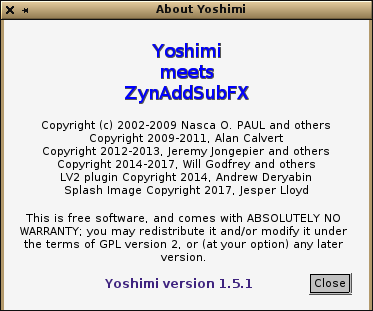
\includegraphics[scale=1.0]{1.5.0/About_1-5-1.png}
   \caption{Yoshimi Menu, About Dialog}
   \label{fig:yoshimi_about_dialog}
\end{figure}

\subsubsection{Menu / Yoshimi / New instance}
\label{subsubsec:menu_yoshimi_new_instance}

   The \textbf{New instance} menu entry creates a new instance of \textsl{Yoshimi}.
   If JACK is running,
   start a normal (JACK-using) instance of \textsl{Yoshimi}.
   Then use this menu entry.  \textsl{Yoshimi} will start another instance
   of itself, with a prompt to accept the next available instance ID or to
   change it.
   The presence of this instance can be verified by running a JACK session
   manager such as QJackCtl.

   In a non-JACK setup it won't fail, but in the absence of any specific
   setting, it will have null audio, but (probably) will still connect to ALSA
   MIDI.  Not too useful, but we should test that sometime.

   It is important to note that each instance of \textsl{Yoshimi} has its
   own configuration file.  Each also has its own MIDI and audio ports.
   Thus, these instances are partly independent of each other.

   The new instance tries to open a \textsl{Yoshimi} instance based on the
   configuration found in the file
   \texttt{\textasciitilde/.config/\-yoshimi/\-yoshimi.configXX}, where
   \textsl{XX} is the ID one supplied.

   Opening a new instance creates a copy that has it's own dynamic memory for
   running storage. In the future, some data (such as recent history) will be
   shared between instances. This will be done only where instances actually
   need to be in sync.

   Each instance has it's own file-store in \textsl{Yoshimi}'s configuration
   directory. The means that if one opens a numbered instance, one will get
   back all the settings that were previously used for that instance.

   Instances no longer fight for access to JACK/ALSA audio; they will simply
   try to find another route to a soundcard. Failing to find one,
   they will revert to null audio, but will nonetheless start cleanly.

   The list of hidden "base parameters" that are set only by the main instance is
   now:

   \begin{itemize}
      \item ALSA Sample Rate
      \item Internal Buffer Size
      \item AddSynth Oscillator Size
      \item XML Compression Level
      \item Show Splash Screen
      \item Enable GUI
      \item Enable CLI
   \end{itemize}

   In the other instances these are now hidden instead of deactivated.  This
   behavior makes sense, as they are \textsl{never} enabled in the other
   instances of \textsl{Yoshimi}. This is more consistent, making
   \textsl{Yoshimi}'s configuration directory more tidy.

\iffalse

%  SECTION COMMENTED OUT

\subsubsection{Menu / Yoshimi / New instance with id...}
\label{subsubsec:menu_yoshimi_new_instance_with_id}

   Creates a new instance of \textsl{Yoshimi}
   with an ID that is a number.
   See \figureref{fig:yoshimi_instance_dialog}.

\begin{figure}[H]
   \centering 
   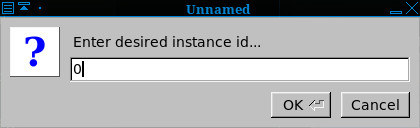
\includegraphics[scale=0.75]{menu/Yoshimi/yoshimi-instance-id.jpg}
   \caption{Yoshimi Menu, Instance Dialog}
   \label{fig:yoshimi_instance_dialog}
\end{figure}

   Useful when connecting devices with JACK.
   Start a normal (JACK-using) instance of \textsl{Yoshimi}.
   Then use this menu entry, supply a number as an ID.
   \textsl{Yoshimi} will start another instance
   of itself, with an ID of whatever number one specified.
   This instance can be verified by running a JACK session manager such as
   \textsl{QJackCtl}.

\fi

\subsubsection{Menu / Yoshimi / Settings...}
\label{subsubsec:menu_yoshimi_settings}

   The \textsl{Yoshimi Settings} dialog contains five tabs that control the
   major and overall settings of \textsl{Yoshimi}.  At the bottom of this
   dialog are two buttons:
   \textbf{Save and Close} and \textbf{Close Unsaved}.
   \index{Save and Close}
   \index{Close Unsaved}

   Please note that the \textbf{Save and Close} and \textbf{Close Unsaved}
   buttons apply to the \textsl{whole}
   \textbf{Settings} window.
   Furthermore, the "saving" does \textsl{not} refer to preserving the changes
   that have been made
   in any of the tabs for the current \textsl{Yoshimi} session.  Any changes
   made in \textbf{Settings} always remain in place for the current
   \textsl{Yoshimi} session.
   However, the changes to the settings are saved to
   the state file \textsl{only} if \textbf{Save and Close} is clicked.

   \setcounter{ItemCounter}{0}      % Reset the ItemCounter for this list.

   \itempar{Save and Close}{Settings!Save and Close}
   This selection saves the settings made in \textbf{all} of the tabs to the
   state file, and closes the \textsl{Yoshimi} settings dialog.

   \itempar{Close Unsaved}{Settings!Close Unsaved}
   Close Unsaved, Main Settings.

   This selection closes the \textsl{Yoshimi} settings dialog.
   However, note that any changes made in the tabs
   \textsl{are preserved}.  They are preserved for the current
   \textsl{Yoshimi} session, but are not saved to the filesystem.

   Here are the tabs included in the main settings of \textsl{Yoshimi}
   as of version 1.4.1; each is described in its own section.

   \begin{itemize}
      \item \textbf{Main settings}
      \item \textbf{Switches}
      \item \textbf{Jack}
      \item \textbf{Alsa}
      \item \textbf{MIDI}
   \end{itemize}

\paragraph{Menu / Yoshimi / Settings / Main Settings}
\label{paragraph:menu_yoshimi_settings_main_settings}

   The Main Settings tab controls the main configuration items that
   follow, which apply to all patches/instruments.
   The main settings are shown in
   \figureref{fig:yoshimi_main_settings_tab}.

   Some settings only take effect after restarting the synthesizer.
   In \textbf{Main settings}, only the two items marked with an asterisk ('*')
   need a restart. 

   The settings dialogs are quite different between \textsl{ZynAddSubFX} and
   \textsl{Yoshimi}.  There are some differences even between
   \textsl{Yoshimi} versions earlier than 1.3.5, and the current version
   (currently 1.3.9).

\begin{figure}[H]
   \centering 
%  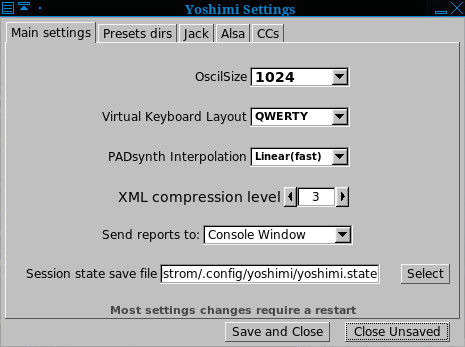
\includegraphics[scale=0.75]{menu/Yoshimi/yoshimi-settings-main.jpg}
%  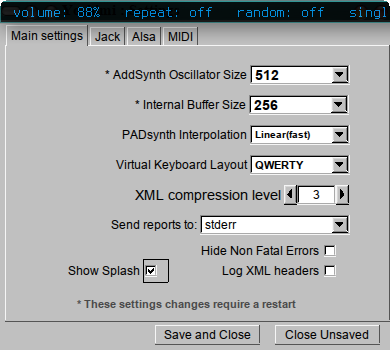
\includegraphics[scale=0.75]{1.3.9/yoshimi-settings-main.png}
   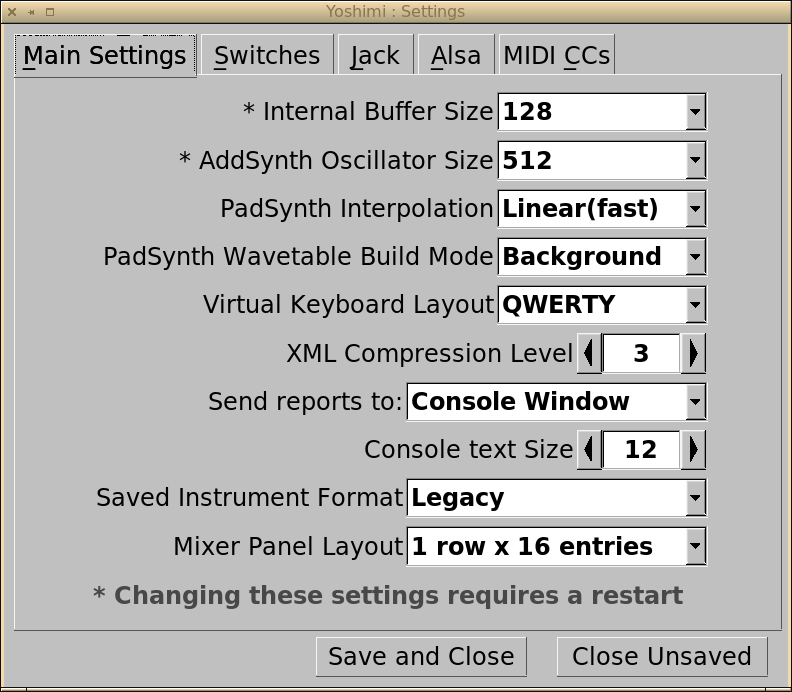
\includegraphics[scale=0.75]{1.4.1/SettingsMain.png}
   \caption{Yoshimi Main Settings Tab}
   \label{fig:yoshimi_main_settings_tab}
\end{figure}

   The following settings exist in the \textsl{Main settings} tab:

   \begin{enumber}
      \item \textbf{AddSynth Oscillator Size}
      \item \textbf{Internal Buffer Size}
      \item \textbf{PADsynth interpolation}
      \item \textbf{Virtual Keyboard Layout}
      \item \textbf{XML compression level}
      \item \textbf{Send reports to}
   \end{enumber}

   \setcounter{ItemCounter}{0}      % Reset the ItemCounter for this list.

   \itempar{AddSynth Oscillator Size}{Main Settings!oscillator size}
   ADDsynth Oscillator Size (in samples).  This item used to be called
   "OscilSize".  Sets the number of the points of the ADDsynth oscillator.
   Bigger is better, but it takes more CPU time on the start of any note, and
   it may add latency to some processes.

   The default value for \textsl{Yoshimi} is shown marked with an asterisk,
   and the default value for \textsl{ZynAddSubFX} is 512.
   \index{asterisk}
   \index{default!asterisk}
   This asterisk/plus-sign convention is used throughout this manual.
   See \figureref{fig:yoshimi_oscilsize_values},
   shown below for the AddSynth Oscillator Size drop-down element.

   Values: \texttt{256, 512*, 1024, 2048, 4096, 8192, 16384}

\begin{figure}[H]
   \centering 
   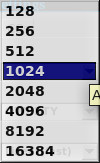
\includegraphics[scale=0.75]{menu/Yoshimi/main-oscilsize.jpg}
   \caption[OscilSize Values]{AddSynth Oscillator Size (samples)}
   \label{fig:yoshimi_oscilsize_values}
\end{figure}

   \itempar{Internal Buffer Size}{Main Settings!buffer size}
   This is a new item for version 1.3.6.  It is actually the old
   \textbf{Period Size} field from the \textbf{Alsa} tab.
   It sets the granularity of the sound generation.
   To find out the internal delay in milliseconds, divide the
   buffer-size value by the sample-rate, then multiply the result by 1000:
   For example, \(256 / 44100 * 1000 = 5.8 ms\).

   The default internal buffer size has been reduced from 1024 to 256.  One
   gets better latency that way.  Almost all modern computers can run
   \textsl{Yoshimi} with the current default (smaller) buffer-size value, and
   many will do so at 64 frames (and even 16 frames!)
   without any special precautions.
   
   Note that, for ALSA, if the audio destination is "default",
   then ALSA decides on the buffer size (among other settings), and
   \textsl{Yoshimi} will set it's internal buffer size to match,
   which always seems to be 1024.

   Values: \texttt{64, 128, 256*, 512, 1024, 2048, 4096}

\begin{figure}[H]
   \centering 
   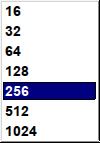
\includegraphics[scale=0.75]{menu/Yoshimi/main-internalsize.jpg}
   \caption[Internal Size Values]{AddSynth Internal Buffer Size (old)}
   \label{fig:yoshimi_internalsize_values}
\end{figure}

   Note that there are two more values, not shown in this old diagram.

   \itempar{PADsynth interpolation}{Main Settings!PADsynth Interpolation}
   See \figureref{fig:padsynth_interpolation}, shown below,
   for the interpolation values.
   From an email conversation with Paul Nasca, Will notes that
   the sound improvement with cubic interpolation is quite subtle, and requires
   a well designed audio setup, a PADsynth instrument with a fair amount of
   high-frequency content... and good hearing!

\begin{figure}[H]
   \centering 
   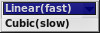
\includegraphics[scale=0.75]{menu/Yoshimi/main-padsynth-interpolation.jpg}
   \caption[PADSynth Interpolation]{PADSynth Interpolation Values}
   \label{fig:padsynth_interpolation}
\end{figure}

   Values: \texttt{Linear(fast)*, Cubic(slow)}

   \itempar{Virtual Keyboard Layout}{Main Settings!Virtual Keyboard Layout}
   The virtual keyboard is useful, but it is difficult to move the mouse
   rapidly to the next key on the virtual keyboard.
   Therefore, \textsl{Yoshimi} supports using the computer keyboard
   to produce notes.

\begin{figure}[H]
   \centering 
   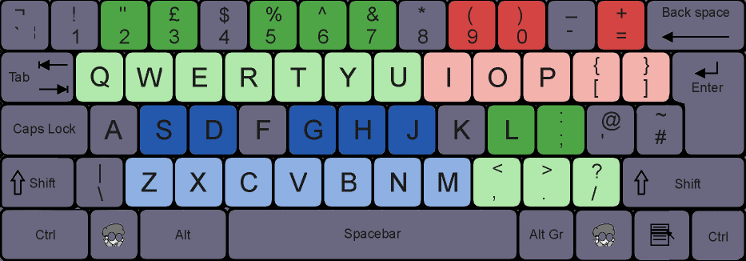
\includegraphics[scale=0.45]{top-panel/ascii-virtual-keyboard.png}
   \caption{QWERTY Virtual Keyboard Layout}
   \label{fig:qwerty_virtual_keyboard}
\end{figure}

   See \figureref{fig:qwerty_virtual_keyboard},
   for the mapping of the computer keyboard to the
   virtual keyboard.
   Three octaves (blue, green, and red) are available, with the dark keys of
   each color representing the "black" keys.
   Note that this is a QWERTY layout.  
   \textsl{Yoshimi} also supports other keyboard layouts.
   See \figureref{fig:virtual_kbd_layout},
   for the virtual keyboard layout settings drop-down.

   Values: \texttt{QWERTY*, Dvorak, QWERTZ, AZERTY}

\begin{figure}[H]
   \centering 
   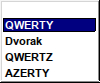
\includegraphics[scale=0.75]{menu/Yoshimi/main-virtual-kbd-layout.jpg}
   \caption[Virtual Keyboard Layout]{Virtual Keyboard Layout Values}
   \label{fig:virtual_kbd_layout} 
\end{figure}

   \itempar{XML compression level}{Main Settings!XML compression level}
   Gzip Compression level of \textsl{Yoshimi} XML files.
   The settings and instruments of
   \textsl{Yoshimi}
   are preserved in XML files.
   The value of 0 indicates that the XML file is uncompressed.

   In general, 0 is probably the best setting for debugging only.  Setting this
   option makes the XML files a bit larger, perhaps larger by a factor of more
   than 10, making a 10K file into a 180K file.  For a little "wasted" space
   and time, one can view the XML file in a text/programmer's editor.  But, if
   one's system is tight on disk space, higher levels of compression can be
   specified.  Using XML compression can also save file access time which may
   be beneficial if one's computer is borderline on latency.  This setting
   should stay at 3 if one is going to save large patchsets that will later be
   loaded while running. Uncompressing is \textsl{much} faster than file
   loading.

   Values: \texttt{0 to 9, 3*}

   \itempar{Send reports to}{Main Settings!Send Reports Destination}
   Notices and error messages can be sent to the standard error log of
   the terminal in which 
   \textsl{Yoshimi} can be run, or, more usefully, to
   an output console window.
   Now these messages are pushed in reverse order, to avoid scrolling
   and to make the most recent statuses easily visible.
   See \figureref{fig:send_reports_to}.
   It provides a depiction of the selection drop-down.

   Values: \texttt{stderr*, Console Window}

\begin{figure}[H]
   \centering 
   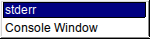
\includegraphics[scale=1.0]{menu/Yoshimi/main-send-reports-to.jpg}
   \caption[Send Reports]{Send Reports To}
   \label{fig:send_reports_to}
\end{figure}

   If the \textbf{Console Window} option is chosen, then the
   \textbf{Reports} button in the effects panel is enabled.
   Pressing the \textbf{Reports} button brings up a small console dialog, as
   shown in \figureref{fig:console_window}.

\begin{figure}[H]
   \centering 
%  \includegraphics[scale=1.0]{1.3.9/console-window.png}
   \includegraphics[scale=1.0]{1.5.0/console-window.png}
   \caption[Yoshimi Console Window]{Console Window}
   \label{fig:console_window}
\end{figure}

    Note that numbers all start from 1 now, although 'specials' (in the command
    line) are still zero-based (they are not seen, though,
    unless set at compile time).

   \index{reports!middle-click}
   An interesting feature of the console window is that one can identify
   user-interface elements of the \textsl{Yoshimi} configuration in this window
   by a middle-click on the user-interface element.
   (Unfortunately, those new single-button touchpads make it impossible to
   provide a middle-click, so one would need a mouse!)

%  The console window figure shows the results of middle-clicking on the
%  following bottom-panel knobs in order:

%  \begin{enumerate}
%     \item Velocity Sense (left-click)
%     \item Velocity Offset
%     \item Pan
%     \item Volume
%  \end{enumerate}

   \index{reports!middle-click}
   Information about each knob middle-clicked is pushed to the top of the
   windows in reverse order.
   \index{reports!left-click}
   \index{reports!right-click}
   Information about an earlier left-click is shown at the bottom of the figure.
   Each left-click ("Button 1") will increase the parameter represented by the
   knob, and each right-click ("Button3") will decrease the parameter
   represented by the knob, and each change is reported in the console window.
   And, of course, each middle-click changes nothing, but reports the current
   value in the console window.
   This feature lets one gather the information needed to
   control the parameter from the command-line.
   The output can be selected, copied, and pasted to a script or archive text
   file for safe-keeping.

%  \index{MIDI learn}
%  Consider it a form of "MIDI learn" that will be developed in the future.
%  And note that it applies to output to \texttt{stderr} as well.

\paragraph{Menu / Yoshimi / Settings / Switches}
\label{paragraph:menu_yoshimi_settings_switches}

   Many of the check-box items have been moved into this new tab, to reduce
   clutter.

\begin{figure}[H]
   \centering 
%  \includegraphics[scale=0.75]{1.4.1/SettingsSwitches.png}
   \includegraphics[scale=0.75]{1.5.0/SettingsSwitches.png}
   \caption{Yoshimi Switches Tab}
   \label{fig:yoshimi_settings_switches_tab}
\end{figure}

   The following settings exist in the \textsl{Switches} tab:

   \begin{enumber}
      \item \textbf{Start With Default State}
      \item \textbf{Hide Non Fatal Errors}
      \item \textbf{Show Splash Screen}
      \item \textbf{Log Load times}
      \item \textbf{Log XML headers}
      \item \textbf{Include disabled data in XML files}
      \item \textbf{Enable GUI}
      \item \textbf{Enable CLI}
   \end{enumber}

   \setcounter{ItemCounter}{0}      % Reset the ItemCounter for this list.

   \itempar{Start With Default State}{Switches!Start With Default State}
   Requires \textsl{Yoshimi} to be restarted, to take effect.
   This setting allows \textsl{Yoshimi} to be initialized with one's own
   initial state file that matches one's usual work setup.
   The default state file is named
   \texttt{\textasciitilde/.config/yoshimi/yoshimi.state}.

   \itempar{Hide Non Fatal Errors}{Main Settings!Hide Non-Fatal Errors}
   Especially when running from the command line (with reports going there
   too), under some circumstances one can get a swamp of low-level error
   messages (such as XRUNs) that is so large that one cannot work out what is
   going on. This feature disables these error messages; it is a work in
   progress to catch the bulk of them, while still reporting top-level messages
   and ones that cause a forced exit (surely not!)

   \itempar{Show Splash Screen}{Main Settings!Show Splash Screen}
   This item will speed up the start-up of \textsl{Yoshimi} slightly
   if unchecked, by not showing the splash screen while files are being loaded.

   \itempar{Log Load times}{Switches!Log Load times}
   Provides a way of noting problematic patch sets, which may take a long
   enough time to load so as to affect the smoothness of playback.

   \itempar{Log XML headers}{Main Settings!Log XML headers}
   This item sends the information to the console window
   (or \texttt{stderr}) so that
   one can then see what \textsl{ynAddSubFX}/\textsl{Yoshimi}
   version created the file.

   \itempar{Include disabled data in XML files}{Main Settings!Include disabled data}
   Allows disabled data to be stored in the XML file.
   This makes it a lot easier to re-enable a setting later.

   \itempar{Enable GUI}{Switches!Enable GUI}
   If checked, the user-interface is enabled.  This setting is normally what you
   want.  If one unchecks it, it warns that disabling the GUI
   can only be reversed from the command line.

   \itempar{Enable CLI}{Switches!Enable CLI}
   If checked, the command-line interface is enabled.
   Note that one cannot disable both the user-interface and the command line
   at the same time.

\paragraph{Menu / Yoshimi / Settings / Jack}
\label{paragraph:menu_yoshimi_settings_jack}

   JACK is the "Jack Audio Connection Kit", very useful for increasing audio
   performance and configurability.
   When using the JACK audio backend, instruments can be individually routed
   and sent to the main L/R outputs. This is controlled from the
   panel window,
   \sectionref{subsec:mixer_panel_window},
   and the settings are saved with all the other parameters.

   Direct part outputs carry the Part and Insertion effects, but not the
   System ones.

\begin{figure}[H]
   \centering 
%  \includegraphics[scale=0.75]{menu/Yoshimi/yoshimi-settings-jack.jpg}
%  \includegraphics[scale=0.75]{1.3.8/yoshimi-settings-jack.jpg}
%  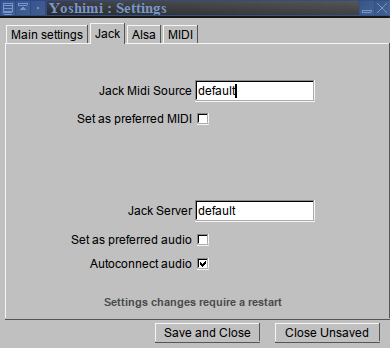
\includegraphics[scale=0.75]{1.3.9/yoshimi-settings-jack.png}
   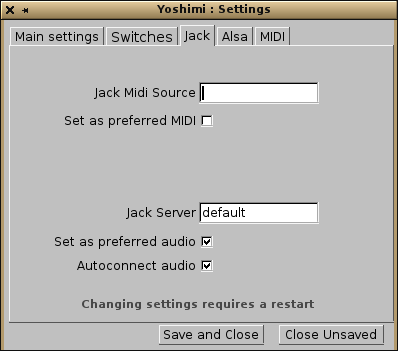
\includegraphics[scale=0.75]{1.4.1/SettingsJack.png}
   \caption[JACK Settings]{JACK Settings Tab}
   \label{fig:yoshimi_settings_jack_tab}
\end{figure}

   The following items are provided by the Jack settings:

   \begin{enumber}
      \item \textbf{Jack Midi Source}
      \item \textbf{Set as preferred MIDI}
      \item \textbf{Jack Server}
      \item \textbf{Set as preferred audio}
      \item \textbf{Autoconnect audio} (new, 1.3.9)
   \end{enumber}

   \setcounter{ItemCounter}{0}      % Reset the ItemCounter for this list.

   \itempar{Jack Midi Source}{JACK!MIDI source}
   Jack MIDI Source.
   It is possible to have more than one JACK MIDI source.  This option
   tells this instance of \textsl{Yoshimi} which JACK
   client to try to auto-connect to for MIDI input.
   This option corresponds to the \textsl{Yoshimi} command line option
   \texttt{--jack-midi(=device)}.

   Values: \texttt{default*, name} name; see "man jackd" for details.

   \itempar{Set as preferred MIDI}{JACK!set as preferred MIDI}
   Set as preferred MIDI for JACK.
   This setting determines which MIDI connections a particular instance will
   first attempt. The switches are mutually exclusive across JACK and ALSA,
   so if one checks ALSA for MIDI, it automatically unchecks JACK for MIDI.
   As well as from the GUI, this setting can be set (for instance 0) from the
   command line, both at start-up and once running.

   \itempar{Jack Server}{JACK!server name}
   Jack Server Name.
   It is possible to have more than one JACK server running.  This option
   tells this instance of \textsl{Yoshimi} which JACK server to use.
   This option corresponds to the \textsl{Yoshimi} command line option
   \texttt{--jack-audio(=server)}.

   Values: \texttt{default*, name} name, as set by
   \texttt{jackd --name}; see "man jackd" for details.

   \itempar{Set as preferred audio}{JACK!set as preferred audio}
   Set as preferred audio for JACK.
   This setting determines which audio connections a particular instance will
   first attempt. The switches are mutually exclusive across JACK and ALSA,
   so if one checks ALSA for audio, it automatically unchecks JACK for audio.
   As well as from the GUI, this setting can be set (for instance 0) from the
   command line, both at start-up and once running.
   Note that any of these setting changes require a restart of \textsl{Yoshimi}
   to take effect.

   \itempar{Autoconnect audio}{JACK!autoconnect audio}
   Sets \textsl{Yoshimi} to connect automatically to the JACK server, just like
   the \texttt{-K} command-line option does.  (However, note that the
   command-line has no way to disable this feature it the configuration has been
   saved.)

\paragraph{Menu / Yoshimi / Settings / Alsa}
\label{paragraph:menu_yoshimi_settings_alsa_tab}

   A significant improvement is to the handling of ALSA audio, which is still
   very important for some people. Until now, \textsl{Yoshimi} has insisted
   on a 2-channel, 16-bit format. Tests have shown that virtually all
   motherboard sound chipsets will handle this, but many external ones don't.

   From \textsl{Yoshimi} 1.3.6 onwards, when using ALSA audio,
   \textsl{Yoshimi} first tries to connect 2 channels at 32 bit depth.  If
   that connection does not succeed, then \textsl{Yoshimi} negotiates
   whatever the soundcard will support.  For example, a card might support
   only 24 bits, and 6 channels.  So \textsl{Yoshimi} will fall back to
   24 bit, and, due to its own limits, will use only channels 1 and 2.
   With external sound modules in mind, endian swaps are also implemented.

   To be able to reliably use ALSA audio, one needs to set a card name, not just
   "Default".  In a terminal window enter the following command:

   \begin{verbatim}
      $ cat /proc/asound/card*/id
   \end{verbatim}

   The result of this command should be something like:

   \begin{verbatim}
      PCH
      K6
   \end{verbatim}

   Go to the ALSA settings tab illustrated below, and in 
   \textsl{Alsa Audio Device} enter, for example, "hw:PCH".
   This ensures one will always connect to this card at startup regardless of
   the order this and other ones.  Another benefit of using this hardware name
   is that ALSA will now use \textsl{Yoshimi}'s internal
   buffer size (256), otherwise ALSA will force \textsl{Yoshimi} to accept its
   default size (usually 1024).

   One can also set the sample rate, but bear in mind that not all cards can use
   all of these.  The sample rates 44100 and 48000 are almost always available.
   If one sets a Midi Device as well (such as a keyboard) Yoshimi will try to
   find and connect to this device at startup.

   To find the MIDI devices available, try:

   \begin{verbatim}
      $ grep Client /proc/asound/seq/clients
   \end{verbatim}

   The result of this command should be something like:

   \begin{verbatim}
      Client info
      Client   0 : "System" [Kernel]
      Client  14 : "Midi Through" [Kernel]
      Client 128 : "TiMidity" [User]
   \end{verbatim}

   It is not obvious how ALSA audio is controlled and who takes command.  If
   one sets a specific audio destination, then \textsl{Yoshimi} makes a
   request.  It's often a negotiation on bit depth and channel count, but
   \textsl{Yoshimi} nearly always gets to decide the buffer size, which is the
   internal buffer size.  However, if the destination is 'default' then ALSA
   decides on the sound card, bit depth, number of channels and the buffer
   size, and \textsl{Yoshimi} will set it's internal buffer size to match.  On
   most machines this seems to be 1024.

\begin{figure}[H]
   \centering 
%  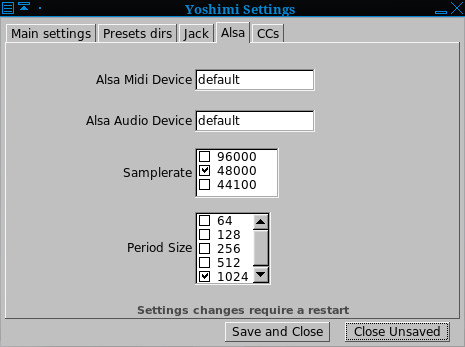
\includegraphics[scale=0.75]{menu/Yoshimi/yoshimi-settings-alsa.jpg}
%  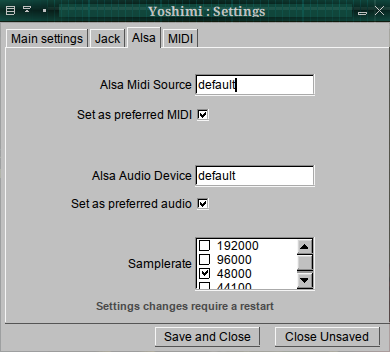
\includegraphics[scale=0.75]{1.3.8/yoshimi-settings-alsa.png}
   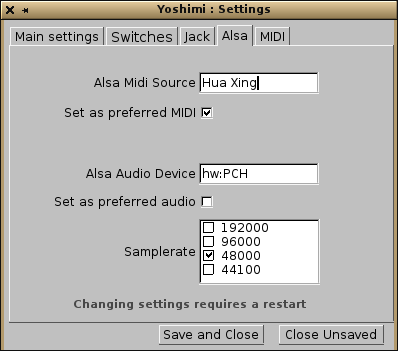
\includegraphics[scale=0.75]{1.4.1/SettingsAlsa.png}
   \caption[ALSA Settings]{ALSA Settings Tab}
   \label{fig:yoshimi_settings_alsa_tab}
\end{figure}

   \setcounter{ItemCounter}{0}      % Reset the ItemCounter for this list.

   \itempar{Alsa Midi Source}{ALSA!MIDI Source}
   ALSA MIDI Source.
   The purpose of this setting is the same as the command line option
   \texttt{--alsa-midi="name"}.
   It is used so that \textsl{Yoshimi} can auto connect to a MIDI source
   such as a keyboard.  For example, the one that Will has identifies itself
   as name = "Hua Xing".
   A port name, such as "128:0" (for one of the ports provided by
   \textsl{TiMidity}) should work as well.
   If the destination is "default",
   then ALSA decides on the sound card, bit depth, number of channels and the
   buffer size, and \textsl{Yoshimi} will set it's internal buffer size to
   match.  On most machines this always seems to be 1024.

   Values: \texttt{default*}

   \itempar{Set as preferred MIDI}{ALSA!Set as preferred MIDI}
   Set as preferred MIDI for ALSA.
   This setting determines which MIDI connections a particular instance will
   first attempt. The switches are mutually exclusive across JACK and ALSA,
   so if one checks ALSA for MIDI, it automatically unchecks JACK for MIDI.
   As well as from the GUI, this setting can be set (for instance 0) from the
   command line, both at start-up and once running.

   \itempar{Alsa Audio Device}{ALSA!audio device}
   ALSA Audio Device.
   This specifies the sound card to which \textsl{Yoshimi} can connect.
   Normally, this will be an ALSA hardware specification such as
   "hw:0".
   ALSA audio also lets one connect to a sound card by name. For example,
   with a Komplete Audio KA 6 sound card, the device specification is
   "hw:K6". This feature is particularly useful for USB modules, as one can
   never be sure where they appear numerically.

   Values: \texttt{default*}

   \itempar{Set as preferred audio}{ALSA!Set as preferred audio}
   Set as preferred audio for ALSA.
   This setting determines which audio connections a particular instance will
   first attempt. The switches are mutually exclusive across JACK and ALSA,
   so if one checks ALSA for audio, it automatically unchecks JACK for audio.
   As well as from the GUI, this setting can be set (for instance 0) from the
   command line, both at start-up and once running.

   \itempar{Samplerate}{ALSA!sample rate}
   Sample Rate.
   Sets the quality of the sound, higher is better, but it uses more CPU.  One
   can select from a list.  Note that both ALSA and JACK will support the
   192000 rate, if the sound-card supports it.  To find out the internal delay
   in milliseconds, divide the buffer-size value by the Sample Rate and
   multiply the result by 1000 (256 / 44100 * 1000 = 5.8 ms).

   Note that, as of version 1.3.6, the \textbf{Period Size} field has been
   removed from the \textbf{Alsa} tab, and is replaced by the 
   \textbf{Internal Buffer Size} field in the \textbf{Main Settings} tab.
   Note that any of these setting changes require a restart of \textsl{Yoshimi}
   to take effect.
   
%  \textsl{ZynAddSubFX}: if one wants a sample-rate that
%  is not in the list, select "Custom" and change the value from the right.
%  Default is 44100.

   Values: \texttt{192000, 96000, 48000*, 44100}

\paragraph{Menu / Yoshimi / Settings / MIDI}
\label{paragraph:menu_yoshimi_settings_ccs}

   The CC settings tab has been renamed the "MIDI" tab.
   This tab, shown in
   \figureref{fig:yoshimi_settings_cc},
   presents MIDI bank-root, bank, program change, and extended program
   change settings, plus some new values.

\begin{figure}[H]
   \centering 
%  \includegraphics[scale=0.75]{menu/Yoshimi/yoshimi-settings-ccs.jpg}
%  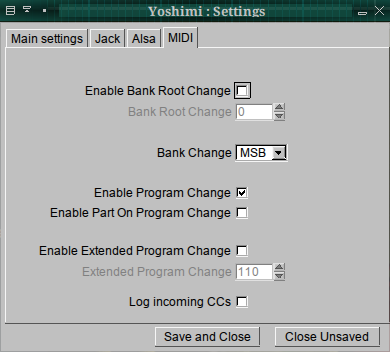
\includegraphics[scale=0.75]{1.3.8/yoshimi-settings-midi.png}
%  \includegraphics[scale=0.75]{1.3.9/yoshimi-settings-ccs.jpg}
%  \includegraphics[scale=0.75]{1.4.1/SettingsMidi.png}
   \includegraphics[scale=0.75]{1.5.0/SettingsMidi.png}
   \caption[MIDI Preferences]{MIDI Preferences Tab}
   \label{fig:yoshimi_settings_cc}
\end{figure}

   A recent feature is that some changes to the items in this
   tab cause a red \textbf{Pending} button to appear.  Pressing this
   button saves that particular change.

\begin{figure}[H]
   \centering 
   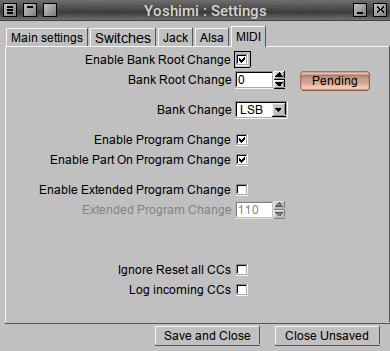
\includegraphics[scale=0.75]{1.4.1/SettingsPending.png}
   \caption[MIDI Settings Pending]{MIDI Settings Pending}
   \label{fig:yoshimi_settings_pending}
\end{figure}

   The following items are provided by the MIDI settings tab:

   \begin{enumber}
      \item \textbf{Enable Bank Root Change}
      \item \textbf{Bank Root Change}
      \item \textbf{Bank Change}
      \item \textbf{Enable Program Change}
      \item \textbf{Enable Part On Program Change}
      \item \textbf{Enable Extended Program Change}
      \item \textbf{Extended Program Change}
      \item \textbf{Ignore Reset all CCs}
      \item \textbf{Log Incoming CCs}
      \item \textbf{Show Learn Editor}
   \end{enumber}

   \setcounter{ItemCounter}{0}      % Reset the ItemCounter for this list.

   The concepts of banks and roots is very useful.
   See \sectionref{subsec:concepts_banks_and_roots}.
   The settings in this tab affect the usage of banks and root changes
   controlled by MIDI messages, thereby making \textsl{Yoshimi} able to
   implement MIDI automation.

   \itempar{Enable Bank Root Change}{MIDI settings!enable bank root change}
   Enable Bank Root Change.

   Values: \texttt{Off*, On}

   \itempar{Bank Root Change}{MIDI settings!bank root change}
   Sets the control value to use for a bank-root change.

   Values: \texttt{0*, to 127}

   If enabled, a new reddish button, \textbf{Pending}, appears.
   Once the change has been made in the scroll list, click this button
   to set the change.
   \textbf{Warning:}
   The \textbf{Save and Close} button will not result in the removal of the
   \textbf{Pending} button.
   This result seems counter-intuitive, but the pending button is not removed
   here because, at that point, it still hasn't actually been either set or
   abandoned. It remains available for when the user actually makes up his/her
   mind.
   If the control number is already in use for
   another purpose, one might get a warning like the following:

\begin{figure}[H]
   \centering 
   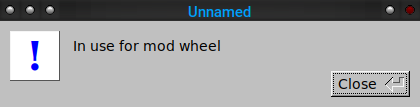
\includegraphics[scale=0.75]{1.5.0/SettingsInUse.png}
   \caption[MIDI Setting In Use]{MIDI Setting In Use}
   \label{fig:yoshimi_settings_in_use}
\end{figure}

   \itempar{Bank Change}{MIDI settings!bank change}
   Bank Change.
   Defines which MIDI settings one wants to use.
   Note that MIDI Controller 0 = CC0 = Bank Select MSB, and MIDI Controller
   32 = CC32 = Bank Select LSB.
   When combined, these Bank Select messages provide \[128*128 = 16384\]
   banks.

   But note that all a Bank Select does is selects the bank for the next
   Program Change event.  The program doesn't change after changing a bank,
   until a Program Change is sent.

   Bank changes can be completely disabled; some hardware
   synthesizers don't play nice with banks.

   Values: \texttt{LSB, MSB*, Off}

   \itempar{Enable Program Change}{MIDI settings!enable program change}

   Values: \texttt{Off*, On}

   Enables/disables MIDI program change.
   Program changes can be completely disabled, but some hardware synths don't
   play nice!

   \itempar{Enable Part On Program Change}{MIDI settings!enable part change}

   Values: \texttt{Off*, On}

   The part is automatically enabled if the MIDI program was changed on this
   part.

   \itempar{Enable Extended Program Change}{MIDI settings!enable extended program change}

   Values: \texttt{Off*, On}

   \itempar{Extended Program Change}{MIDI settings!extended change}
   If enabled, a new reddish button, \textbf{Pending}, appears.
   Once the change has been made in the scroll list, click this button
   to set the change.

   Values: \texttt{0-127, 110*}

   \itempar{Ignore Reset all CCs}{MIDI settings!Ignore Reset all CCs}
   Causes \textsl{Yoshimi} to ignore this message.
   \index{CC monitor}
   For example, using \textsl{Yoshimi}'s fairly new CC monitor (see the next
   item), Will found that \textsl{Rosegarden} was sending CC 121 (reset all
   controllers) at the start of some song segments.  Checking this option
   prevents unwanted resets.

   Values: \texttt{Off*, On}

   \itempar{Log Incoming CCs}{MIDI settings!Log Incoming CCs}
   This setting is now saved (in the \texttt{config} file). It is there
   as an aid for when \textsl{Yoshimi} appears to ignore MIDI commands,
   as it tells one exactly what \textsl{Yoshimi} thinks it received.

   Values: \texttt{Off*, On}

   \itempar{Show Learn Editor}{MIDI settings!Show Learn Editor}
   Sets whether the MIDI Learn editor window is to be opened when learning a
   new control. One might find that when learning a new control one
   usually wants to change the \textbf{Min} and \textbf{Max} settings.

   Values: \texttt{Off, On*}

\subsubsection{Menu / Yoshimi / MIDI Learn...}
\label{subsubsec:menu_yoshimi_midi_learn}

   The \textbf{MIDI Learn} functionality of \textsl{Yoshimi} gives it the
   ability to redirect MIDI input from physical controllers to various
   user-interface controls in \textsl{Yoshimi}, so that the user can basically
   control \textsl{Yoshimi}'s knobs and sliders via MIDI equipment.

   There's enough to say about this topic so that we describe it in a section
   of its own.
   See \sectionref{sec:midi_learn} for details.

\subsubsection{Menu / Yoshimi / Exit}
\label{subsubsec:menu_yoshimi_exit}

   Simply exits from \textsl{Yoshimi}.
   The user is prompted if unsaved changes exist, as shown in
   \figureref{fig:yoshimi_change_exit}.

   One can sometimes get a false parameters-changed warning if one
   scrolls through one of the menu type entries without actually changing it.
   Better safe than sorry!

\begin{figure}[H]
   \centering 
   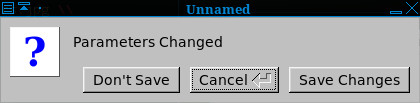
\includegraphics[scale=0.75]{menu/Yoshimi/yoshimi-menu-exit-parameters-changed.jpg}
   \caption[Yoshimi Menu, Exit]{Yoshimi Menu, Exit}
   \label{fig:yoshimi_change_exit}
\end{figure}

% We moved some out-of-date menu entries into the following document, and
% created additional sub-sections to include, with up-to-date information.
%
% %-------------------------------------------------------------------------------
% yum_menu
%-------------------------------------------------------------------------------
%
% \file        yum_menu_instruments.tex
% \library     Documents
% \author      Chris Ahlstrom
% \date        2015-05-11
% \update      2016-02-27
% \version     $Revision$
% \license     $XPC_GPL_LICENSE$
%
%     Provides the Menu section of yoshimi-user-manual.tex.
%
%-------------------------------------------------------------------------------

\subsection{Menu / Instruments}
\label{subsec:menu_instrument}

   The \textsl{Yoshimi} Instruments menu lets one select instruments and work
   with banks of instruments.
   \textsl{Yoshimi} stamps instrument XML files with its own major and minor
   version numbers so it is possible to tell which version created the files,
   or whether they were created by \textsl{ZynAddSubFX}.

   When opening an instrument bank one can now tell exactly which synth engines
   are used by each instrument. This is represented by three pale background
   colours:

   \begin{itemize}
      \item \textcolor{red}{Red}: ADDsynth
      \item \textcolor{blue}{Blue}: SUBsynth
      \item \textcolor{green}{Green}: PADsynth
   \end{itemize}

   These new colored engine backgrounds aren't just pretty. They give real
   information about expected processor load, and time taken to be ready when
   loaded:

   \begin{itemize}
      \item \textsl{Processor Load, low to high}: PAD, SUB, then ADD.
      \item \textsl{Time to initialize, low to high}: SUB, ADD, PAD.
   \end{itemize}

   If the instruments are kits they scanned to find out if 
   \textsl{any} member of the kit contains each engine.
   This scanning is duplicated in the current part, the mixer panel for the
   currently loaded instruments, and in the Instrument Edit window the same
   colors highlight the engine names when they are enabled with the check
   boxes. 

   The following sub-menus are provided, as shown in
   \figureref{fig:yoshimi_instrument_menu}.

\begin{figure}[H]
   \centering 
   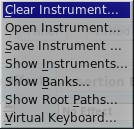
\includegraphics[scale=1.0]{1.3.8/yoshimi-menu-instrument.jpg}
   \caption{Yoshimi Menu, Instrument}
   \label{fig:yoshimi_instrument_menu}
\end{figure}

   TODO:  Document the many differences in 1.3.8 here.

   \begin{enumber}
      \item \textbf{Clear Instrument...}
      \item \textbf{Open Instrument...}
      \item \textbf{Save Instrument...}
      \item \textbf{Show Instruments...}
      \item \textbf{Show Banks...}
      \item \textbf{Show Root Paths...}
   \end{enumber}

   These menu entries don't appear in the order in which they would normally
   be used.  For simplicity, it is better, especially for \textsl{Yoshimi}
   1.3.5 and above, to summarize how to navigate through these menu items,
   before showing each one in detail.

   \setcounter{ItemCounter}{0}      % Reset the ItemCounter for this list.

   \itempar{Set Current Root Path}{root!set current}
   \index{root!current}
   Instruments are stored in banks, and banks are stored in root directories,
   also known as "roots".  In \textsl{Yoshimi}, there can be a number of
   roots that exist in a user's directory structure, but only one root can be
   the current root.  Thus, the first step is to set up the current root
   directory to point to where we have stored all our banks of instruments.

   \begin{enumber}
      \item In \textsl{Yoshimi}, navigate to the \textbf{Instrument / Show
      Root Paths...} entry in the main menu.
      \item In the \textbf{Bank Root Paths} dialog, select the desired
      bank path by clicking on it.
      \item Click the \textbf{Make Current} button.
%     \item Then click the \textbf{Open Current} button.
      \item Then click the \textbf{Save and Close} button.
   \end{enumber}

   For example, one can make the \texttt{/usr/share/yoshimi/banks} directory
   the current root directory.  This directory is the default location for
   banks when \textsl{Yoshimi} is first installed.
   In the following figure, we set it to the author's local directory,
   \texttt{~/Audio/yoshimi/banks}.
   In general, it is recommended that one copies the default installed
   directories to a local directory, in order to be able to work with them,
   making additions and changes without needing root permissions, and
   without risking the corruption of the default installation.

   For figures and details about the \textbf{Show Root Paths...} menu entry,
   see \sectionref{subsubsec:menu_instrument_show_root_paths}.

   \itempar{Show Current Bank Set}{banks!show}
   Once the current root has been set, one can then see all of the banks
   under that root.  Navigate to the \textbf{Instrument / Show Banks...} menu
   entry and click it.  This brings up a dialog such as the one shown in
   \figureref{fig:show_ca_banks}.  That dialog shows all of the banks that
   exist in the current root directory.  Each is auto-numbered by
   \textsl{Yoshimi} the first time that root directory is accessed, and the
   current bank is highlighted in pink.

   Clicking on a bank with both make that bank the current bank, and opens an
   instruments dialog, such as that shown in
   \figureref{fig:show_alex_j_bank}.

   \itempar{Show Instruments in Current Bank}{instruments!show}
   Once the current root and current bank have been set, another way to show
   the instruments is to navigate to the
   \textbf{Instrument / Show Instruments...} menu entry and click on it.
   Again, this action opens an instruments dialog, such as that shown in
   \figureref{fig:show_alex_j_bank}.

   A left-click on a particular instrument sets that instrument into the
   current Part in force in the main \textsl{Yoshimi} window, where it can
   then be edited, if desired.

   \index{anti-auto-clutter}
   Right-clicking on an instrument causes the instruments list dialog
   to disappear, and be replaced by an instrument dialog.  While this
   behavior might be surprising, it is part of the anti-auto-clutter feature
   of \textsl{Yoshimi}.

   Now that we know how to easily navigate through roots, banks, and
   instruments, we can discuss each of the \textbf{Instrument} menu entries
   in detail.

\subsubsection{Menu / Instrument / Clear Instrument...}
\label{subsubsec:menu_instrument_clear}

   This menu entry brings up a prompt to clear the parameters of the
   instrument that is currently loaded in the current part.

\begin{figure}[H]
   \centering 
   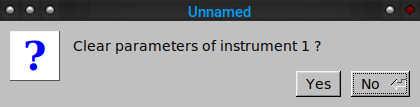
\includegraphics[scale=0.75]{menu/Instrument/clear-instrument.jpg}
   \caption{Clear Instrument Dialog}
   \label{fig:clear_instrument_dialog}
\end{figure}

   \textbf{Bug:}
   \index{bugs!need to clear instrument?}
   Sometime it seems that one needs to clear the instrument if one is
   loading a new instrument to test it out, because some settings seem
   to remain from the previous instrument.

   \textsl{Don't quote us on that.  Maybe Will has fixed that issue by now.}

\subsubsection{Menu / Instrument / Open Instrument...}
\label{subsubsec:menu_instrument_open}

   This menu entry brings up a prompt to open a new instrument.
   This prompt is a file-dialog, and it doesn't depend at all on the settings
   of the current root or the current bank.  It does have a
   \textbf{Favorites} button to help the user get quickly to the desired
   location of instrument files.

\begin{figure}[H]
   \centering 
   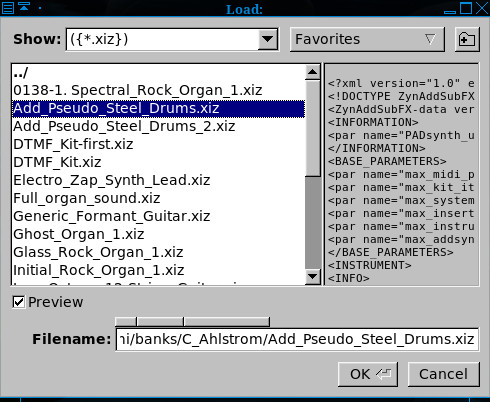
\includegraphics[scale=0.75]{menu/Instrument/open-instrument.jpg}
   \caption{Open Instrument Dialog}
   \label{fig:open_instrument_dialog}
\end{figure}

   This dialog has a number of user-interface elements to discuss.

   \begin{enumber}
      \item \textbf{Show}
      \item \textbf{Favorites}
      \item \textbf{Create a new diretory}
      \item \textbf{Instrument List}
      \item \textbf{XML Preview}
      \item \textbf{Preview}
      \item \textbf{Show hidden files}
      \item \textbf{Directory Bar}
      \item \textbf{Filename}
      \item \textbf{OK}
      \item \textbf{Cancel}
   \end{enumber}

   \setcounter{ItemCounter}{0}      % Reset the ItemCounter for this list.

   \itempar{Show}{Open Instrument!show}
   Show types of files.
   This item shows a file filter for selecting instrument files.
   The types of filters are as follows (screen shot not available):

   \begin{enumber}
      \item \textbf{(\{*.xiz\})} (compressed XML files)
      \item \textbf{All Files (*)}
      \item \textbf{Custom Filter}
   \end{enumber}

   \itempar{Favorites}{Open Instrument!favorites}
   Favorite directories.
   Provides a list of options and favorite directories in which to find 
   instrument files.

\begin{figure}[H]
   \centering 
   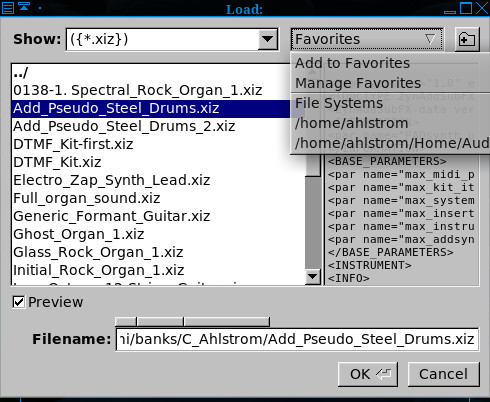
\includegraphics[scale=0.75]{menu/Instrument/favorites-dropdown.jpg}
   \caption{Favorites Drop-down}
   \label{fig:open_instrument_favorites}
\end{figure}

   \begin{enumber}
      \item \textbf{Add to Favorites}
      \item \textbf{Manage Favorites}
      \item \textbf{File Systems}
      \item \textbf{(Additional favorite directories)}
   \end{enumber}

   \index{Add to Favorites}
   \textbf{Add to Favorites}
   simply adds the currently selected directory shown in the instrument list
   to the list of favorites.

   To add Favorites in the file dialog, navigate to the desired directory.
   Then click \textbf{Favorites}, and select \textbf{Add to Favorites}.

   Once one has a number of favorites set up,
   there is a \textbf{Manage Favorites} that can be used.
   For example, if one needs to get rid of a directory, one can use the
   \textbf{Manage Favorites}
   \index{Manage Favorites}
   dialog, shown in
   \figureref{fig:manage_instrument_favorites} below,
   to do that.

\begin{figure}[H]
   \centering 
   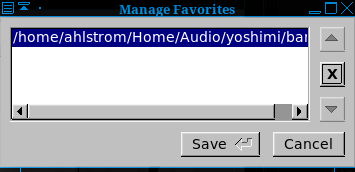
\includegraphics[scale=1.0]{menu/Instrument/manage-favorites.png}
   \caption{Favorites Drop-down}
   \label{fig:manage_instrument_favorites}
\end{figure}

   \textbf{File Systems} \index{File Systems}
   Provides a list of all file systems starting at root ("\texttt{/}").
   This list can be pretty confusing, with a lot of entries.
   But note that one navigates to ("\texttt{/}"), and from there to
   \texttt{/usr/share/yoshimi/banks} to get easy access to all the
   instruments that are preinstalled with
   \textsl{Yoshimi}.
   Generally, one will want to use only
   \textbf{Add to Favorites} and \textbf{Manage Favorites}.

   \itempar{Create Directory}{Open Instrument!create new directory}
   Creates a New Directory.
   This little symbol options a small "New Directory?" dialog (not shown
   here, it is very simple and stock) into which one can type a directory
   name to be added to the current directory of the instrument list.

   \itempar{Instrument List}{Open Instrument!instrument list}
   Provides a list of the instrument files available in the current
   directory.  Also shown are sub-directories (if available)
   that might contain more instruments, and a ("\texttt{../}") entry
   to navigate to the parent directory.

   \itempar{Preview}{Open Instrument!preview checkbox}
   If one thinks the preview feature is not useful, uncheck this check-box.
   so that one doesn't see the preview window.  As a bonus, one can see more
   of the instrument file-name.

   \itempar{Preview pane}{Open Instrument!preview pane}
   XML Preview.
   This box can show the beginning of the XML data of an instrument file.
   \textbf{Bug:}
   \index{bugs!compressed XML preview}
   It seems to show the XML only if the XML is not compressed.

   \itempar{Show hidden files}{Open Instrument!show hidden files}
   Shows file that are hidden.  Not sure how useful this feature is;
   who would hide a \textsl{Yoshimi} instrument file?

   \itempar{Directory Bar}{Open Instrument!directory bar}
   Provides an alternate way to move up through the directory structure.

   \itempar{Filename}{Open Instrument!filename}
   File Name.
   Provides the full path to the instrument file.

   \itempar{OK/Cancel}{Open Instrument!ok/cancel}
   We don't really need to discuss the \textbf{OK} and \textbf{Cancel}
   buttons, do we?

\subsubsection{Menu / Instrument / Save Instrument...}
\label{subsubsec:menu_instrument_save}

   This menu entry brings up a prompt to save a new instrument within the
   user's file system.
   It has all of the user-interface elements of the "Open Instrument"
   dialog shown in
   \figureref{fig:open_instrument_dialog}
   in \sectionref{subsubsec:menu_instrument_open}.
   Like that dialog, it is not dependent on the current root or current bank.
   However, if nothing has changed, then a "Nothing to Save!" prompt (not
   pictured) is shown.

   With \textsl{ZynAddsubFX} and older versions of \textsl{Yoshimi},
   it was possibly to end up with unnamed instruments. Since version
   1.3.4, \textsl{Yoshimi} will trap such an occurrence and name it
   'No Title'; it will not let one save the unedited default sound.

\subsubsection{Menu / Instrument / Show Instruments...}
\label{subsubsec:menu_instrument_show}

   Instruments are stored in banks. The banks (and current bank setting)
   are loaded/saved
   automatically by the program, so one doesn't have to worry about saving the
   banks before the program exits. On program start, the last used bank is
   loaded. A single bank can store up to 128 instruments. 
   However, there is space for a number of additional
   instruments in the bank, the extended-program section, to allow up to 160
   instruments in a bank.

   When the \textbf{Show Instruments...} button is selected, a dialog comes
   up that shows all of the instruments present in the currently-selected
   bank.
   
\begin{figure}[H]
   \centering 
   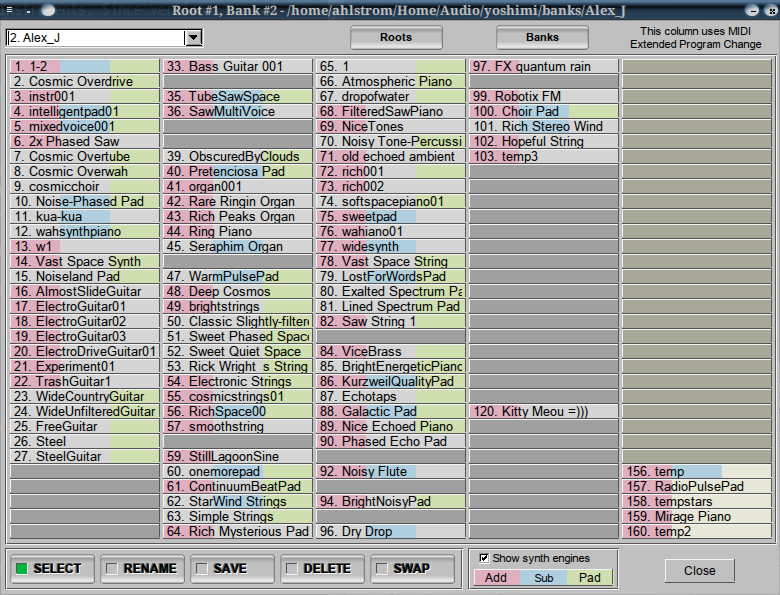
\includegraphics[scale=0.75]{1.3.6/Alex_J_bank_instruments.png}
   \caption[Instruments in Current Bank]{Instruments in Current Bank 1.3.6}
   \label{fig:show_alex_j_bank}
\end{figure}

   As \figureref{fig:show_alex_j_bank}
   shows, this is a very complex dialog with a lot of options.
   Note how \textsl{Yoshimi} now shows the color codings for the
   synth-sections used in each instrument:
   red for ADDsynth, blue for SUBsynth, and
   green for PADsynth.

   Also note how the numbers at the beginning of the filenames are used as
   an "instrument" or "program" number.  These numbers can be used in MIDI
   Program Change commands.
   
   All of the files with filenames starting with 4-digit numbers will be
   shown in the slot corresponding number.  Those without numbers will start
   with numbers at 129 or above ("extended program change").  One should give
   them numbers by renaming them outside of \textsl{Yoshimi}, then reloading
   the bank.

   \index{extended program}
   Note that MIDI CC
   (see \sectionref{paragraph:menu_yoshimi_settings_ccs})
   can be set to access voices from 129 to 160.
   All the Bank controls in the \textbf{MIDI} settings tab take immediate
   effect when set.
   Bank and program changes can be completely disabled in the settings tab;
   some hardware synths don't play nice with it.

   Learning how to use the Instruments dialog is an important way to make
   instruments easier to manage, and so this will be a long discussion.

%  An important pair of concepts in \textsl{Yoshimi} are
%  \textsl{banks} and \textsl{roots}.  These concepts are described in
%  \sectionref{subsec:concepts_banks_and_roots}.

%  A bank has 3 modes in \textsl{ZynAddSubFX}: 

%  \begin{enumber}
%     \item \textbf{READ}.
%        The instrument is loaded from the bank to the current part.
%     \item \textbf{WRITE}.
%        The instrument is written to the bank.
%     \item \textbf{CLEAR}.
%        The instrument from the bank is cleared (removed).
%  \end{enumber}

%  Pressing the left mouse button on a slot reads/writes/clears the
%  instrument from/to it (according to the current mode).
   
%  Pressing the right mouse button on a slot changes its name.

%  The setup in \textsl{Yoshimi} is a bit different than in
%  \textsl{ZynAddSubFX}.
%  Observe \figureref{fig:show_ca_bank}.
%  It shows a bank loaded from a directory containing customs
%  banks from one of the authors of this document.

   Note that this dialog has been modified in recent versions of
   \textsl{Yoshimi}.

   Here is a list of the user-interface items in the instruments/banks dialog.

   \begin{enumber}
      \item \textbf{Bank Names}
      \item \textbf{Roots}
      \item \textbf{Banks}
      \item \textbf{Instrument and Bank Matrix}
      \item \textbf{SELECT}
      \item \textbf{RENAME}
      \item \textbf{SAVE}
      \item \textbf{DELETE}
      \item \textbf{SWAP}
      \item \textbf{Show synth engines}
         (was \textbf{Show PADsynth status})
      \item \textbf{Close}
   \end{enumber}

   \setcounter{ItemCounter}{0}      % Reset the ItemCounter for this list.

   \itempar{Bank Names}{instruments!bank names}
   Instruments Bank Name.
   Basically, each bank is a directory name, with a number prepended.
   The banks are found under the current root, which is a also a directory
   name, and is the name of the parent directory of a set of banks.
   Here is the Bank Names drop-down list for "my" setup, which has the
   default banks plus a lot of banks found around the Internet:

\begin{figure}[H]
   \centering 
   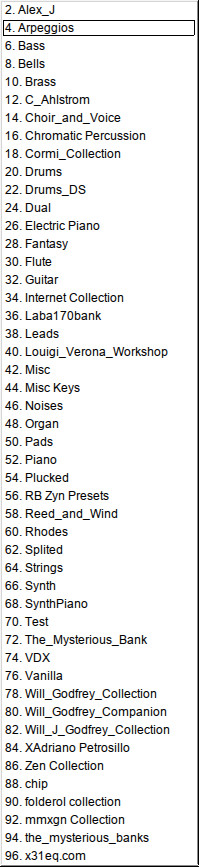
\includegraphics[scale=0.75]{menu/Instrument/bank-list.jpg}
   \caption[A Sample Bank List]{A Sample Bank List}
   \label{fig:bank_list}
\end{figure}

   And here is the directory listing associated with it, in the order
   produced by the UNIX/Linux "ls -1" (list single-column) command (shown in
   two columns to save space):

   \begin{verbatim}
      Alex_J                        Noises
      Arpeggios                     Organ
      Bass                          Pads
   '  Bells                         Piano
      Brass                         Plucked
      C_Ahlstrom                    RB Zyn Presets
      chip                          README
      Choir_and_Voice               Reed_and_Wind
      Chromatic Percussion          Rhodes
      Cormi_Collection              Splited
      Drums                         Strings
      Drums_DS                      Synth
      Dual                          SynthPiano
      Electric Piano                Test
      Fantasy                       The_Mysterious_Bank
      Flute                         the_mysterious_banks
      folderol collection           Vanilla
      Guitar                        VDX
      Internet Collection           Will_Godfrey_Collection
      Laba170bank                   Will_Godfrey_Companion
      Leads                         Will_J_Godfrey_Collection
      Louigi_Verona_Workshop        x31eq.com
      Misc                          XAdriano Petrosillo
      Misc Keys                     Zen Collection
      mmxgn Collection
   \end{verbatim}

   The first thing to note is that there are only 128 \textsl{Yoshimi} banks
   supported in a \textsl{Yoshimi} root.  The list above takes up about half
   of the available slots, so it might be time to move some of those banks
   to a new root directory.

   The numbers in the drop-down list are generated by \textsl{Yoshimi} the
   first time it sees a new root path or a new bank within the root path.
   Once set, these numbers will never change unless one actually moves them
   around (using the \textbf{SWAP} button).

   The bank number is also the MIDI ID for the bank;
   one can be sure that it will always
   be there for bank changes, no matter how many banks are added later.
   \textsl{Yoshimi} always lists the banks in ID order, not alphabetical
   order, so one can group them sensibly and permanently.
   However, at first-time creation \textsl{Yoshimi} sets the IDs in
   alphabetical order and tries to space them evenly over the range to
   provide some wiggle room.                                        

   Selecting one of the items in this drop-down list selects the bank and
   loads it into the Banks dialog.

   \index{anti-auto-clutter}
   Right-clicking on a bank causes the banks list dialog
   to disappear, and be replaced by the bank dialog.  While this
   behavior might be surprising, it is part of the anti-auto-clutter feature
   of \textsl{Yoshimi}.

   \itempar{Roots}{instruments!roots}
   Instruments Roots Button.
   Shows a list of directories that can serve as "root" directories.
   The "Bank Root Paths" dialog shown in
   \figureref{fig:show_banks_roots} shows
   the system root (e.g. \texttt{/usr/share/yoshimi/banks}) and
   a user's home location for his/her banks and roots.

   \itempar{Banks}{instruments!banks}
   Banks Button.
   This item brings up a Banks dialog showing all of the banks present in the
   current root.
   It is an alternative to using the \textbf{Bank Names} dropdown list.

   \itempar{Instrument and Bank Matrix}{instruments!bank matrix}
   Instruments Bank Matrix.
   Shows the instruments that are in the currently selected bank
   (directory).

   \itempar{SELECT}{instruments!SELECT}
   Instruments SELECT.
   When this button is selected, then clicking on an instrument selects that
   instrument as the instrument for the current Part active in the main
   window.

   \itempar{RENAME}{instruments!RENAME}
   Instruments RENAME.
   When this button is selected, then clicking on a bank brings
   up a small dialog to rename the clicked-on bank.
   However, one might also experience the following warning message:

   \begin{verbatim}
      This instrument file cannot be changed
   \end{verbatim}

   \itempar{SAVE}{instruments!SAVE}
   Instruments SAVE.
   When this button is selected, then clicking on a bank saves
   the instruments as currently configured.
   However, one might also experience the following warning message:

   \begin{verbatim}
      This instrument file cannot be changed
   \end{verbatim}

   \itempar{DELETE}{instruments!DELETE}
   Instruments DELETE.
   Selecting this button and clicking an empty bank entry does nothing.
   Selecting this button and clicking an existing bank entry brings up a
   small dialog asking one if this bank is really to be deleted.
   However, one might also experience the following warning message:

   \begin{verbatim}
      This instrument file cannot be changed
   \end{verbatim}

   \itempar{SWAP}{instruments!SWAP}
   Instruments SWAP.
   Selecting this button, then selecting one bank, and then another,
   swaps the numbering and postion of the selected banks.
   However, one might also experience the following warning message:

   \begin{verbatim}
      This instrument file cannot be changed
   \end{verbatim}

   \itempar{Show synth engines}{instruments!show engines}
   If enabled, then the usage of each of the \textsl{Yoshimi} synthesis
   engines is indicated by color coding, as shown in the figure above.

   \itempar{Close}{instruments!Close}
   Closes the window.

   Here is a more conventional view of instruments, supplied with
   \textsl{Yoshimi}, shown in
   \figureref{fig:show_pads_bank}.

\begin{figure}[H]
   \centering 
%  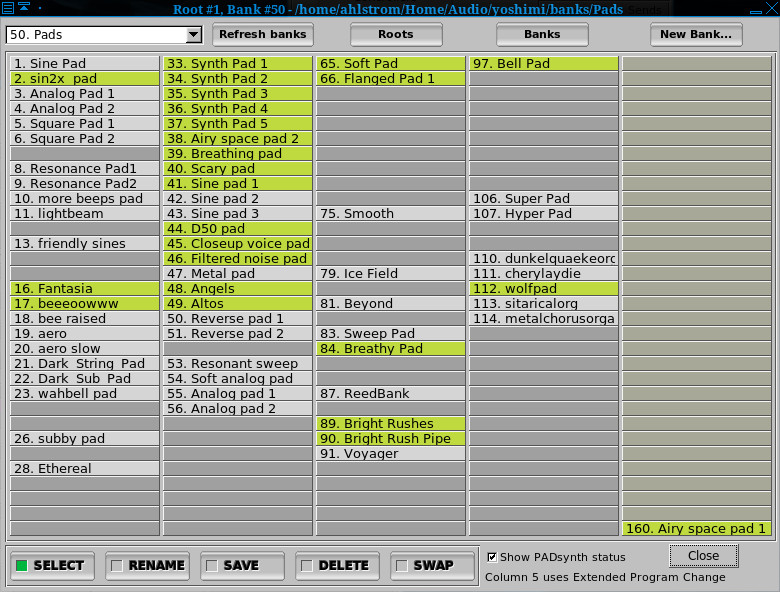
\includegraphics[scale=0.75]{menu/Instrument/show-pads-bank.jpg}
   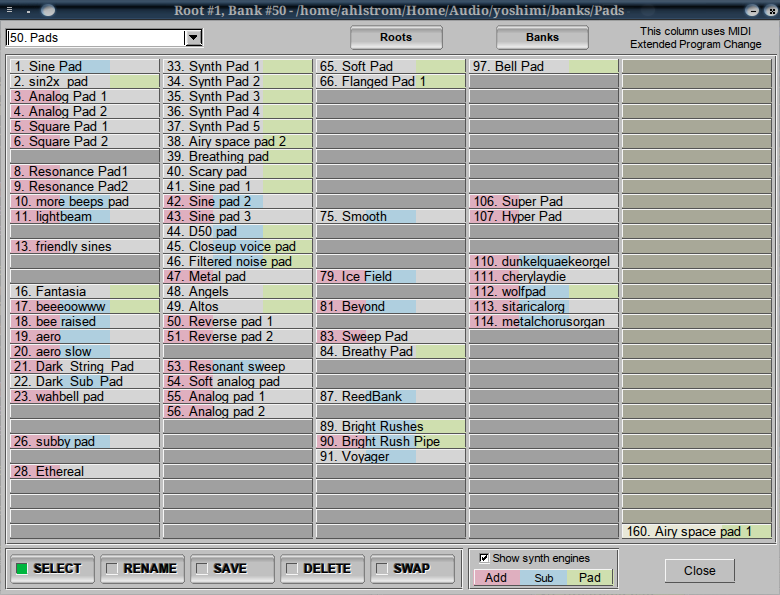
\includegraphics[scale=0.75]{1.3.6/show_pads_bank.png}
   \caption[Show Pads Instruments]{Show Pads Instruments}
   \label{fig:show_pads_bank}
\end{figure}

   Note that many of these Pads instruments also use the Add and Sub
   components as well.

\subsubsection{Menu / Instrument / Show Banks...}
\label{subsubsec:menu_instrument_show_banks}

   This menu entry brings up a dialog that shows all of the banks present in
   the current root.

\begin{figure}[H]
   \centering 
   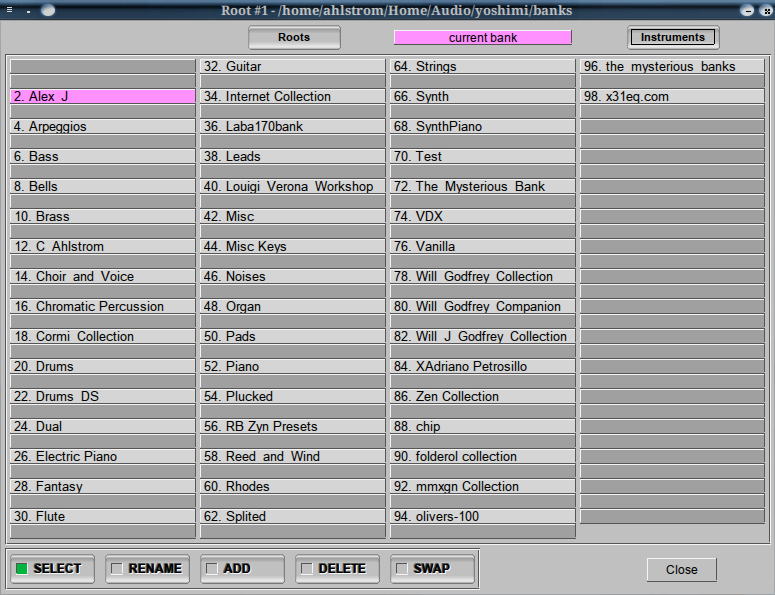
\includegraphics[scale=0.75]{1.3.6/show_CA_banks.png}
   \caption[Show Banks]{Show Banks in Current Root}
   \label{fig:show_ca_banks}
\end{figure}

   This figure illustrates a setup where the installed banks were combined with
   banks downloaded from various web sites.
   The following list shows that the interface elements in the banks dialog
   are slightly different from the instruments dialog.

   \begin{enumber}
      \item \textbf{Roots}
      \item \textbf{Current Bank} (passive display element)
      \item \textbf{Instruments}
      \item \textbf{SELECT}
      \item \textbf{RENAME}
      \item \textbf{ADD}
      \item \textbf{DELETE}
      \item \textbf{SWAP}
      \item \textbf{Close}
   \end{enumber}

   \setcounter{ItemCounter}{0}      % Reset the ItemCounter for this list.

   \itempar{Roots}{banks!roots}
   Banks Roots.
   "Roots" button.
   Shows a list of directories that can serve as "root" directories.

   \itempar{current bank}{banks!current bank}
   \index{current!bank}
   Current Bank.  Simply indicates the current bank via color-highlighting.
   Note that one can left-click on a bank in this dialog to make it the
   current bank.  This setting is saved across \textsl{Yoshimi} restarts.

   \itempar{Instruments}{banks!instruments}
   Banks Instruments.
   \index{current!bank}
   Brings up a banks dialog that shows the instruments in the current bank.

   \itempar{SELECT}{banks!SELECT}
   Banks SELECT.
   When this button is selected, then clicking on a bank makes it the current
   bank.

   (Although we don't show a figure for it, note that some banks provide
   instruments with numbers in the extended program-change range (above
   127) prepended to the file-names.)

   \itempar{RENAME}{banks!RENAME}
   Banks RENAME.
   When this button is selected, then clicking on a bank brings
   up a small dialog to rename the clicked-on bank.
   However, one might also experience the following warning message:

   \begin{verbatim}
      This bank directory cannot be changed
   \end{verbatim}

   \itempar{ADD}{banks!ADD}
   Banks ADD.
   Selecting this button and clicking an empty bank entry brings up a small
   dialog to create a new empty bank name for that entry.
   If one clicks on an existing bank entry, then a small dialog comes up
   stating that the bank number selected is already in use.
   However, one might also experience the following warning message:

   \begin{verbatim}
      This bank directory cannot be changed
   \end{verbatim}

   \itempar{DELETE}{banks!DELETE}
   Banks DELETE.
   Selecting this button and clicking an empty bank entry does nothing.
   Selecting this button and clicking an existing bank entry brings up a
   small dialog asking one if this bank is really to be deleted.
   However, one might also experience the following warning message:

   \begin{verbatim}
      This bank directory cannot be changed
   \end{verbatim}

   \itempar{SWAP}{banks!SWAP}
   Banks SWAP.
   Selecting this button, then selecting one bank, and then another,
   swaps the numbering and postion of the selected banks.
   This button is good for minor reorganization of the bank numbers.

\subsubsection{Menu / Instrument / Show Root Paths...}
\label{subsubsec:menu_instrument_show_root_paths}

\begin{figure}[H]
   \centering 
   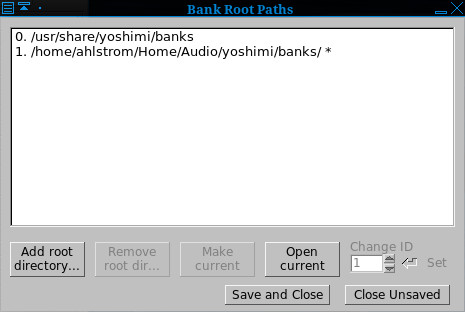
\includegraphics[scale=0.75]{menu/Instrument/show-banks-roots.jpg}
   \caption[Show Root Paths]{Show Root Paths}
   \label{fig:show_banks_roots}
\end{figure}

   \setcounter{ItemCounter}{0}      % Reset the ItemCounter for this list.

   \itempar{Add root directory...}{Root Paths!add directory}
   Show Root Paths Add Root Directory.
   To add a bank root path:

   \textsl{Yoshimi} (as installed by Debian Linux) provides a default bank at
   \texttt{/usr/share/yoshimi/banks}.
   To add one's own directory, navigate to "Yoshimi / Instrument / Show Root
   Paths ...".  Then click on "Add root directory...".

   Once selected, one will see that \texttt{/usr/share/yoshimi/banks}
   is marked with an asterisk.  One can select the new root directory,
   and make it current by clicking the "Make current" button.
   Then the Banks dialog will show all the banks in that directory, one bank
   per subdirectory (each subdirectory "is" a bank).

\begin{figure}[H]
   \centering 
   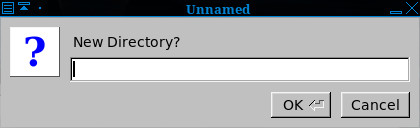
\includegraphics[scale=0.75]{menu/Instrument/new-directory.jpg}
   \caption{Add Root Directory}
   \label{fig:add_root_directory}
\end{figure}

   \itempar{Remove root directory...}{Root Paths!remove directory}
   Show Root Paths Remove Root Directory.
   If a path is selected, then this button is active, and can be used to
   delete the selected path from the "root paths" list.

   \itempar{Make current}{Root Paths!make current}
   Show Root Paths Make Current.
   \index{current!root}
   This button marks the currently-selected path as the "current root" path.

   \itempar{Open current}{Root Paths!open current}
   Show Root Paths Open Current.
   This button opens the current root path.

   \itempar{Change ID}{Root Paths!change ID}
   Show Root Paths Change ID.

   Values: \texttt{0* to 127}

   \textsl{
   We need to know more about how this ID can be used.
   Is it a way to make the path selectable via an extended MIDI control, or
   some other automation method?
   }

%-------------------------------------------------------------------------------
% vim: ts=3 sw=3 et ft=tex
%-------------------------------------------------------------------------------


%-------------------------------------------------------------------------------
% yum_menu_instruments
%-------------------------------------------------------------------------------
%
% \file        yum_menu_instruments.tex
% \library     Documents
% \author      Chris Ahlstrom
% \date        2016-02-27
% \update      2018-12-29
% \version     $Revision$
% \license     $XPC_GPL_LICENSE$
%
%     Provides the Menu / Instruments section of the manual.
%
%-------------------------------------------------------------------------------

\subsection{Menu / Instruments}
\label{subsec:menu_instrument}

   The \textsl{Yoshimi} Instruments menu lets one select instruments and work
   with banks of instruments.

   While the \textbf{Instrument Menu} allows for the management of parts, the
   \textbf{Part Edit} dialog, described in
   \sectionref{subsec:bottom_panel_instrument_edit},
   is where one would start for the the creation of a new part/instrument.

   When opening an instrument bank one can now tell exactly which synth engines
   are used by each instrument. This is represented by three pale background
   colours:

   \begin{itemize}
      \item \textbf{\textcolor{red}{Red}}: ADDsynth
      \item \textbf{\textcolor{blue}{Blue}}: SUBsynth
      \item \textbf{\textcolor{green}{Green}}: PADsynth
   \end{itemize}

   These new coloured engine backgrounds aren't just pretty. They give real
   information about expected processor load, and time taken to be ready when
   loaded:

   \begin{itemize}
      \item Processor Load, low to high:
         \textbf{\textcolor{green}{PAD}},
         \textbf{\textcolor{blue}{SUB}}, then
         \textbf{\textcolor{red}{ADD}}.
      \item Time to initialise, low to high:
         \textbf{\textcolor{blue}{SUB}},
         \textbf{\textcolor{red}{ADD}},
         \textbf{\textcolor{green}{PAD}}.
   \end{itemize}

   If the instruments are kits they are scanned to find out if
   \textsl{any} member of the kit contains each engine.
   This scanning is duplicated in the current part, the mixer panel for the
   currently loaded instruments, and in the Instrument Edit window the same
   colours highlight the engine names when they are enabled with the check
   boxes.

   The following sub-menus are provided, as shown in
   \figureref{fig:yoshimi_instrument_menu}.

\begin{figure}[H]
   \centering
   \includegraphics[scale=0.9]{1.6.0/menu_instrument.png}
   \caption{Yoshimi Menu, Instruments}
   \label{fig:yoshimi_instrument_menu}
\end{figure}

   This new version of the \textbf{Instruments}
   menu is somewhat different than
   the old version.  It is actually simpler and easier to use, while still
   offering all of the power of the setting up of instruments in
   \textsl{Yoshimi}.

   \begin{enumber}
      \item \textbf{Show Stored...}
      \item \textbf{Load External...}
      \item \textbf{Save External...}
      \item \textbf{Recent Instruments...}
      \item \textbf{Clear}
      \item \textbf{Search}
   \end{enumber}

%  \setcounter{ItemCounter}{0}      % Reset the ItemCounter for this list.

\subsubsection{Menu / Instrument / Show Stored...}
\label{subsubsec:menu_instrument_show}

   Instruments are stored in banks
   (see \sectionref{subsec:concepts_banks_and_roots}).
   The banks (and current bank setting) are
   loaded/saved automatically by the program, so one doesn't have to worry
   about saving the banks before the program exits. On program start, the last
   used bank is loaded. A single bank can store up to 128 instruments.
   However, there is space for a number of additional instruments in the bank,
   the extended-program section, to allow up to 160 instruments in a bank.

   When the \textbf{Show Stored...} button is selected, a dialog comes
   up that shows all of the instruments present in the currently-selected
   bank.

\begin{figure}[H]
   \centering
   \includegraphics[scale=0.75]{2.3.0/instruments.png}
   \caption[Show Stored Instruments]{Instruments Stored in Current Banks}
   \label{fig:instruments_show_stored}
\end{figure}

   As \figureref{fig:instruments_show_stored},
   shows, this is a very complex dialog with a lot of options.
   The figure shows a default setup, with the bank of instruments at location
   30, \textbf{30. Misc}, listed.
   If one drops this list down (shown later), one also observes that the banks
   are numbered in increments of 5, to make it easier for a user to insert his
   or her own bank(s) of instruments. The default set of banks are spaced 5
   apart for this reason. If we add more than 25 banks in future versions of
   \textsl{Yoshimi}, then a \textsl{clean} install will wrap round starting with
   location 2 and again spaced 5 apart, and so-on until all spaces are filled.
   For an existing setup, new entries will just be slotted in where they
   will fit.

   Also, if one deletes banks or instruments by some external means, the next
   time \textsl{Yoshimi} starts, it will notice their absence and quietly
   remove their entries.

   Note how \textsl{Yoshimi} shows the colour coding for the
   synth-sections used in each instrument:
   red for ADDsynth, blue for SUBsynth, and green for PADsynth.
   This used to be switchable as not fetching the colour information from the
   banks meant startup was sometimes slightly faster. However this then
   interfered with later developments that use this information for other
   purposes so it has now been removed.

   Also note how the numbers at the beginning of the filenames are used as
   an "instrument" or "program" number.  These numbers can be used in MIDI
   Program Change commands.

\index{new!Instrument Highlight}
   A new feature since \textsl{Yoshimi} V 1.7.2 is highlighting the last
   instrument seen. In this case, the third one in the list. This is
   particularly useful for banks where the internal name is different from the
   filename.

   All of the instrument files (such as \texttt{0001-Arpeggio1.xiz})
   with filenames starting with numbers (no matter how many digits)
   will be shown in the corresponding slot number.
   Variations in filename after the number are ignored; the files
   are treated as the same instrument.

   Those instrument files
   without numbers (or larger numbers?) will start
   with numbers at 129 or above ("Extended Program Change") up to 160.
   One could give them numbers by renaming them outside of \textsl{Yoshimi},
   then reloading the bank.
   One can also fix unnumbered ones simply by loading them, then re-saving them
   to the same slot. It's then probably best to swap them into the main set,
   if there is space.

   \index{extended program}
   Note that MIDI CC
   (see \sectionref{paragraph:menu_yoshimi_settings_ccs})
   can be set to access voices from 129 to 160.
   All the Bank controls in the \textbf{MIDI} settings tab take immediate
   effect when set.
   Bank and program changes can be completely disabled in the settings tab;
   some hardware synths don't play nice with it.

   Learning how to use the Instruments dialog is an important way to make
   instruments easier to manage, and so this will be a long discussion.

%  An important pair of concepts in \textsl{Yoshimi} are
%  \textsl{banks} and \textsl{roots}.  These concepts are described in
%  \sectionref{subsec:concepts_banks_and_roots}.

   Here is a list of the user-interface items in the instruments/banks dialog:

   \begin{enumber}
      \item \textbf{Bank Names}
      \item \textbf{Search}
      \item \textbf{Roots}
      \item \textbf{Banks}
      \item \textbf{Instrument and Bank Matrix}
      \item \textbf{SELECT}
      \item \textbf{RENAME}
      \item \textbf{SAVE}
      \item \textbf{DELETE}
      \item \textbf{SWAP}
%      \item \textbf{Show synth engines}
      \item \textbf{Close}
   \end{enumber}

   \setcounter{ItemCounter}{0}      % Reset the ItemCounter for this list.

   \itempar{Bank Names}{instruments!bank names}
   Instruments Bank Name.
   This item is a drop-down list of the available instrument banks in the
   currently-selected \textbf{root} directory.
   Basically, each bank is a directory name, with a number prepended.
   The banks are found under the current root, which is a also a directory
   name, and is the name of the parent directory of a set of banks.
   Here is the Bank Names drop-down list for the default setup, which has the
   default banks provided by the basic \textsl{Yoshimi} installation.

\begin{figure}[H]
   \centering
%  \includegraphics[scale=0.75]{menu/Instrument/bank-list.jpg}
   \includegraphics[scale=0.75]{2.3.0/banks.png}
   \caption[A Sample Bank List]{A Sample Bank List}
   \label{fig:bank_list}
\end{figure}

   And here is the directory listing associated with it, in the order
   produced by the UNIX/Linux \texttt{ls -1}
   (list single-column) command (shown in
   two columns to save space):

   \begin{verbatim}
      Arpeggios          Plucked
      Bass               Reed_and_Wind
      Brass              Rhodes
      Choir_and_Voice    Splited
      Drums              Strings
      Dual               Synth
      Fantasy            SynthPiano
      Guitar             The_Mysterious_Bank
      Misc               Will_Godfrey_Collection
      Noises             Will_Godfrey_Companion
      Organ              chip
      Pads               Cormi_Sound
   \end{verbatim}

   The directories (banks) shown above come from the default \textbf{root}
   when \textsl{Yoshimi} and its data files are installed:

   \begin{verbatim}
      /usr/share/yoshimi/banks
   \end{verbatim}

   If one installed \textsl{Yoshimi} by building the source code, then
   this directory is:

   \begin{verbatim}
      /usr/local/share/yoshimi/banks
   \end{verbatim}

   Note that the directory that holds the banks is shown in the title bar.
   Another good source of banks, if one installs \textsl{ZynAddSubFX}, is:

   \begin{verbatim}
      /usr/share/zynaddsubfx/banks
   \end{verbatim}

   Note that there are only 128 \textsl{Yoshimi} banks
   supported in a \textsl{Yoshimi} root.
   If the list of banks takes up about half of the available slots, it might be
   time to move some of those banks to a new root directory.

   The numbers in the drop-down list are generated by \textsl{Yoshimi} the
   first time it sees a new root path or a new bank within the root path.
   Once set, these numbers will never change unless one actually moves them
   around (using the \textbf{SWAP} button).

   The bank number is also the MIDI ID for the bank;
   one can be sure that it will always
   be there for bank changes, no matter how many banks are added later.
   \textsl{Yoshimi} always lists the banks in ID order, not alphabetical
   order, so one can group them sensibly and permanently.
   However, at first-time creation \textsl{Yoshimi} sets the IDs in
   alphabetical order and tries to space them evenly over the range to
   provide some wiggle room.
   Selecting one of the items in this drop-down list selects the bank and
   loads it into the Banks dialog.

   \index{anti-auto-clutter}
   Right-clicking or left-clicking on a bank in the drop-down list
   causes the instrument list of the previous bank to be replaced by the
   instrument list of the newly-selected bank.

   \index{new!instruments search}
   \itempar{Search}{instruments!search}
   Instruments Search Button.
   This feature arrived with \textsl{Yoshimi} V 1.6.0 and provides a
   way of finding instruments of a given type right across all known banks and
   bank roots.


\begin{figure}[H]
   \centering
%  \includegraphics[scale=0.75]{menu/Instrument/bank-list.jpg}
   \includegraphics[scale=0.5]{2.3.0/search.png}
   \caption[A search list List]{A search list}
   \label{fig:bank_search}
\end{figure}
   The top field is a drop-down menu that gives all the types
   \textsl{Yoshimi} recognises, and below this is the list of those
   most recently found. As well as the names of the instruments
   one sees the bank root ID, bank ID and instrument number. All of these
   are the values that will be recognised by MIDI.

   Clicking on any entry will immediately load the instrument into the
   current part \textbf{without} changing the settings for current bank or
   root.

   \itempar{Roots}{instruments!roots}
   Instruments Roots Button.
   Shows a list of directories that can serve as "root" directories.
   The "Bank Root Paths" dialog discussed in
   \sectionref{subsubsec:menu_patch_sets_patch_bank_roots}\hspace{4pt}in
   \figureref{fig:show_patch_banks}\hspace{4pt}shows
   the system root (e.g. \texttt{/usr/share/yoshimi/banks}) and
   a user's home location for his/her banks and roots.

   \itempar{Banks}{instruments!banks}
   Banks Button.
   This item brings up a Banks dialog showing all of the banks present in the
   current root.
   It is an alternative to using the \textbf{Bank Names} drop-down list to
   select a bank.  It is also a way to reorganise and renumber the
   banks without using the Linux console or a file-explorer application to do
   so.

   \itempar{Instrument and Bank Matrix}{instruments!bank matrix}
   Instruments Bank Matrix.
   Shows the instruments that are in the currently selected bank.

   The next few items are selector buttons that determine what happens when one
   clicks on an instrument name.

   \itempar{SELECT}{instruments!SELECT}
   Instruments SELECT.
   When this button is selected, then clicking on an instrument selects that
   instrument as the instrument for the current Part active in the main
   window.  In the main window of \textsl{Yoshimi}, that instrument name will
   appear in the currently-selected \textbf{Part}.  If \textsl{Yoshimi} is
   writing to a console window then each part, when clicked, will be shown:

   \begin{verbatim}
		yoshimi> Loaded 64 "Hyper Organ1" to Part 1
		Loaded 65 "Hyper Arpeggio" to Part 1
		Loaded 10 "Arpeggio11" to Part 1
		Loaded 41 "Soft Arpeggio4" to Part 1
		Loaded 67 "Glass Arpeggio1" to Part 1
   \end{verbatim}

   \itempar{RENAME}{instruments!RENAME}
   Instruments RENAME.
   When this button is selected, then clicking on a bank brings
   up a small dialog to rename the clicked-on bank.
   However, one will see the following warning message if trying to rename a
   file that is in a directory not modifiable by normal users:

   \begin{verbatim}
      ! Could not rename instrument 39 to Soft Arpeggio5 [Close]
   \end{verbatim}

   Note that, as soon as this operation is done, the auto-selector (green
   check-box) moves back to the \textbf{SELECT} button.

   \itempar{SAVE}{instruments!SAVE}
   Instruments SAVE.
   When this button is selected, then clicking on a bank saves
   the instruments as currently configured.
   A prompt like the following will appear:

   \begin{verbatim}
      ? Overwrite the slot no. 43 ?  [No/Yes]
   \end{verbatim}

   However, if one answers yes, and the instrument is in a non-modifiable
   directory, then one will see the following error message:

   \begin{verbatim}
      ! Could not save to this location [Close]
   \end{verbatim}

   \itempar{DELETE}{instruments!DELETE}
   Instruments DELETE.
   Selecting this button and clicking an empty bank entry does nothing.
   Selecting this button and clicking an existing bank entry brings up a
   small dialog asking one if this bank is really to be deleted.

   \begin{verbatim}
      ? Clear the slot no. 68?  [No/Yes]
   \end{verbatim}

   However, if one answers yes, and the instrument is in a non-modifiable
   directory, then one will see the following error message:

   \begin{verbatim}
      ! Could not clear this location  [Close]
   \end{verbatim}

   \itempar{SWAP}{instruments!SWAP}
   Instruments SWAP.
   Selecting this button, then selecting one instrument, and then another,
   swaps the numbering and position of the selected instruments.
   However, one might also experience the following warning message:

   \begin{verbatim}
      ! Could not swap these locations  [Close]
   \end{verbatim}

   Note that all of the above error messages are also shown in the console, if
   it is where \textsl{Yoshimi} is running.  For example:

   \begin{verbatim}
      40 Failed to remove /usr/local/share/yoshimi/banks/Arpeggios/0041-Soft
      Arpeggio3.xiz Permission denied
   \end{verbatim}

%   \itempar{Show synth engines}{instruments!show engines}
%   If enabled, then the usage of each of the \textsl{Yoshimi} synthesis
%   engines is indicated by color coding, as shown in the figure above.

%   \textbf{Note} This also affects the new search feature, as at startup there
%    is a scan of all banks checking for the instrument engines and type.

   \itempar{Close}{instruments!Close}
   Closes the window.

%  Here is a more conventional view of instruments, supplied with
%  \textsl{Yoshimi}, shown in
%  \figureref{fig:show_pads_bank}.
%
% \begin{figure}[H]
%    \centering
% %  \includegraphics[scale=0.75]{menu/Instrument/show-pads-bank.jpg}
%    \includegraphics[scale=0.75]{1.3.6/show_pads_bank.png}
%    \caption[Show Pads Instruments]{Show Pads Instruments}
%    \label{fig:show_pads_bank}
% \end{figure}
%
%    Note that many of these Pads instruments also use the Add and Sub
%    components as well.

\subsubsection{Menu / Instrument / Load External...}
\label{subsubsec:menu_instrument_load}

   This menu entry simply brings up a file dialog, allowing the user to
   navigate to an arbitrary directory, and then to a solitary instrument file
   (\texttt{*.xiz}), and load it into the current Part.

\begin{figure}[H]
   \centering
   \includegraphics[scale=0.5]{2.3.0/filer.png}
   \caption{Instruments, Load External}
   \label{fig:instruments_load_external}
\end{figure}

   These "xiz" files are normally found in a \texttt{banks} directory, but
   this operation allows access to instruments that are not located in a bank.

   \begin{itemize}
      \item If loading an external instrument file with no internal name,
         the file leafname will be shown.
      \item If loading an external instrument file with the name
         \textsl{Simple Sound}, the name \textsl{No Title} will be given.
      \item If loading a patch set that has unnamed instruments, or ones with
         the name \textsl{Simple Sound}, those will be given the name \textsl{No
         Title}.
   \end{itemize}

   This dialog has a number of user-interface elements to discuss:

   For further details see \sectionref{subsec:interface_filer}.

\iffalse
   \begin{enumber}
      \item \textbf{Show}
      \item \textbf{Favorites}
      \item \textbf{Create a new directory}
      \item \textbf{Instrument List}
      \item \textbf{XML Preview}
      \item \textbf{Preview}
      \item \textbf{Show hidden files}
      \item \textbf{Directory Bar}
      \item \textbf{Filename}
      \item \textbf{OK}
      \item \textbf{Cancel}
   \end{enumber}

   These elements are used in a number of different places in
   \textsl{Yoshimi}.
   Therefore, we will explain them all once, here.

   \setcounter{ItemCounter}{0}      % Reset the ItemCounter for this list.

   \itempar{Show}{Load External!show}
   Show types of files.
   This item shows a file filter for selecting instrument files.
   The types of filters are as follows (screen shot not available):

   \begin{enumber}
      \item \textbf{(\{*.xiz\})} (compressed XML files)
      \item \textbf{All Files (*)}
      \item \textbf{Custom Filter}
   \end{enumber}

   \itempar{Favorites}{Load External!favorites}
   Favourite directories.
   Provides a list of options and favourite directories in which to find
   instrument files.

\begin{figure}[H]
   \centering
   \includegraphics[scale=0.75]{menu/Instrument/favorites-dropdown.jpg}
   \caption{Manage Favorites Drop-Down List}
   \label{fig:open_instrument_favorites}
\end{figure}

   \begin{enumber}
      \item \textbf{Add to Favorites}
      \item \textbf{Manage Favorites}
      \item \textbf{File Systems}
      \item \textbf{\textsl{(current favourite directories)}}
   \end{enumber}

   \index{Add to Favorites}
   \textbf{Add to Favorites}
   simply adds the currently selected directory shown in the instrument list
   to the list of favourites.

   To add favourites in the file dialog, navigate to the desired directory.
   Then click \textbf{Favorites}, and select \textbf{Add to Favorites}.

   Once one has a number of favourites set up,
   there is a \textbf{Manage Favorites} that can be used.
   For example, if one needs to get rid of a directory, one can use the
   \textbf{Manage Favorites}
   \index{Manage Favorites}
   dialog, shown in
   \figureref{fig:manage_instrument_favorites} below,
   to do that.

\begin{figure}[H]
   \centering
   \includegraphics[scale=0.75]{menu/Instrument/manage-favorites.png}
   \caption{Manage Favorites Dialog}
   \label{fig:manage_instrument_favorites}
\end{figure}

   \textbf{File Systems} \index{File Systems}
   Provides a list of all file systems starting at root ("\texttt{/}").
   This list can be pretty confusing, with a lot of entries.
   But note that one navigates to ("\texttt{/}"), and from there to
   \texttt{/usr/share/yoshimi/banks} to get easy access to all the
   instruments that are preinstalled with
   \textsl{Yoshimi}.
   Generally, one will want to use only
   \textbf{Add to Favorites} and \textbf{Manage Favorites}.

   \itempar{Create Directory}{Load External!create new directory}
   Creates a New Directory.
   This little symbol brings up a small "New Directory?" dialog (not shown
   here, it is very simple and stock) into which one can type a directory
   name to be added to the current directory of the instrument list.

   \itempar{Instrument List}{Load External!instrument list}
   Provides a list of the instrument files available in the current
   directory.  Also shown are sub-directories (if available)
   that might contain more instruments, and a ("\texttt{../}") entry
   to navigate to the parent directory.

   \itempar{Preview}{Load External!preview checkbox}
   If one thinks the preview feature is not useful, uncheck this check-box.
   so that one doesn't see the preview window.  As a bonus, one can see more
   of a long instrument file-name.

   \itempar{Preview pane}{Load External!preview pane}
   XML Preview.
   This box can show the beginning of the XML data of an instrument file.
   \textbf{Bug:}
   \index{bugs!compressed XML preview}
   The XML preview feature shows the XML only if the XML is not compressed.

   \itempar{Show hidden files}{Load External!show hidden files}
   Shows file that are hidden.  Not sure how useful this feature is;
   who would hide a \textsl{Yoshimi} instrument file?

   \itempar{Directory Bar}{Load External!directory bar}
   Provides an alternate way to move up through the directory structure.
   Click on each of the small bevelled rectangles to move around in the
   directory hierarchy.

   \itempar{Filename}{Load External!filename}
   File Name.
   Provides the full path specification for the instrument file.

   \itempar{OK/Cancel}{Load External!ok/cancel}
   We don't really need to discuss the \textbf{OK} and \textbf{Cancel}
   buttons, do we?  OK, we'll cancel that discussion.
\fi
\subsubsection{Menu / Instrument / Save External...}
\label{subsubsec:menu_instrument_save}

   This menu entry simply brings up a file dialog, allowing the user to
   navigate to an arbitrary directory, and then save the current Part
   to a solitary instrument file (\texttt{*.xiz}).

\begin{figure}[H]
   \centering
   \includegraphics[scale=0.75]{2.3.0/save_ext_instrument.png}
   \caption{Instruments, Save External}
   \label{fig:instruments_save_external}
\end{figure}

   This dialog is very similar to the \textbf{Load External} dialog.
%   Note the large question mark in the XML preview, indicating a compressed XML
%   file.  If uncompressed, then an XML text preview will be shown.

   The instrument save action saves only what is essential to the instrument,
   and not the part it may be sitting in.  If there have been no changes in the
   instrument, then a \textbf{Nothing to save!} dialog appears.

   From \textsl{Yoshimi} V1.7.4 there is a warning if the 'type' filed has
   not been filled in. One can ignore this and save regardless, but it is
   hoped the gentle reminder will encourage more people to fill it in.

\subsubsection{Menu / Instrument / Recent Instruments...}
\label{subsubsec:menu_instrument_recent}

   This menu brings up a simple window with a list of the most recent
   instruments that have been selected.  A single-click on the desired
   instrument will load it.

\subsubsection{Menu / Instrument / Clear}
\label{subsubsec:menu_instrument_clear}

   Normally this menu entry simply clears the instrument that is loaded into
   the current Part.  This converts the instrument to a
   \textsl{Simple Sound} patch.
   However, if the Ctrl key is held down when clicking on the entry, the entire
   part will be returned to default values, including Controllers etc.

   In either case, the menu entry brings up a prompt with details of exactly what
   will be cleared.

\begin{figure}[H]
   \centering
   \includegraphics[scale=0.75]{2.3.0/clear_instrument.png}
   \caption{Clear Instrument Dialog}
   \label{fig:clear_instrument_dialog}
\end{figure}
\begin{figure}[H]
   \centering
   \includegraphics[scale=0.75]{2.3.0/clear_part.png}
   \caption{Clear Part Dialog}
   \label{fig:clear_part_dialog}
\end{figure}

   \textbf{No} is the default action.

\subsubsection{Menu / Instrument / Search}
\label{subsubsec:menu_instrument_search}

   This entry provides a quicker route to the instrument search feature described
   in \sectionref{subsubsec:menu_instrument_show}
\subsubsection{Menu / Instrument / Misc Notes}
\label{subsubsec:menu_instrument_misc_notes}

   There are still many instruments out there with
   no internal title. This fact applies to both external files and instruments
   in banks, and means that, once loaded, one does not know what instruments
   one has. So now, if the internal name is missing, \textsl{Yoshimi} will use
   the leaf-name of the file.  When one saves an instrument to a bank slot, it
   will get a filename with the internal name as the leaf-name.  When saving
   an instrument to an external file, the first offered will be the internal
   name and in the current directory, but this can be changed if desired.

   The part and mixer name fields will always show the (possibly adjusted)
   internal name regardless of the external filename, which could easily have
   been changed at some time.  The instrument banks will always show the file's
   leaf-name, so it more-or-less matches external files (what one sees from a
   file display).  As soon as one edits an instrument, if it was \textsl{Simple
   Sound}, the name will be changed to \textsl{No Title}.  \textsl{Yoshimi}
   generally won't let one rename an instrument to \textsl{Simple Sound}.

   Default instruments are never saved, not even in patch sets and states, but
   if the parts are activated, that fact \textsl{is} saved; it's a part
   feature, not an instrument one.

   Patch sets will save all other instruments regardless of whether they are
   activated or not.

   While testing all these features, Will created a new multi-part instrument
   kit.  It's now in the \textsl{Companion} set and is called \textsl{Pad Kit}.

%-------------------------------------------------------------------------------
% vim: ts=3 sw=3 et ft=tex
%-------------------------------------------------------------------------------


%-------------------------------------------------------------------------------
% yum_menu_patch_sets
%-------------------------------------------------------------------------------
%
% \file        yum_menu_patch_sets.tex
% \library     Documents
% \author      Chris Ahlstrom
% \date        2016-02-27
% \update      2018-03-11
% \version     $Revision$
% \license     $XPC_GPL_LICENSE$
%
%     Provides the Menu / Instruments section of yoshimi-user-manual.tex,
%     for the 1.3.8 and above versions of Yoshimi.  That menu entry has changed
%     a lot.
%
%-------------------------------------------------------------------------------

\subsection{Menu / Patch Sets}
\label{subsubsec:menu_patch_sets}

   This new menu entry is part of the very nice reorganization and simplification
   of the handling of roots and banks in the new \textsl{Yoshimi}.  The
   \textbf{Patch Sets} menu replaces the old \textbf{Parameters} menu.  Do you
   like the new name?  The patch set saves all of the settings, including effects
   and instruments.  Patch sets will save all other instruments regardless of
   whether they are activated or not.  Default instruments are never saved, not
   even in patch sets, but if the parts are activated that fact \textsl{is}
   saved.  It is a part feature, not an instrument feature.

   \textsl{Yoshimi} stamps its configuration XML files with its own major and
   minor version numbers so it is possible to tell which version created the
   files, or whether they were created by \textsl{ZynAddSubFX}.

   The main dialog is somewhat similar in layout and function to the
   dialog shown in
   \figureref{fig:instruments_show_stored},
   for managing instruments in a selected bank.

\subsubsection{Menu / Patch Sets / Show Patch Banks...}
\label{subsubsec:menu_patch_sets_show_patch_banks}

   The \textbf{Banks} window has had some button shuffling, and one can
   import and export banks as well.

\begin{figure}[H]
   \centering 
%  \includegraphics[scale=0.75]{menu/Instrument/show-banks-roots.jpg}
%  \includegraphics[scale=0.75]{1.3.9/patch_sets_show_patch_banks.png}
   \includegraphics[scale=0.75]{1.5.7/Bank.png}
   \caption[Show Patch Banks]{Show Patch Banks}
   \label{fig:show_patch_banks}
\end{figure}

   Here is a list of the user-interface items in the patch-banks dialog:

   \begin{enumber}
      \item \textbf{Roots}
      \item \textbf{current bank}
      \item \textbf{Instruments}
      \item \textbf{Bank Matrix}
      \item \textbf{SELECT}
      \item \textbf{RENAME}
      \item \textbf{SAVE}
      \item \textbf{DELETE}
      \item \textbf{SWAP}
      \item \textbf{IMPORT}
      \item \textbf{EXPORT}
      \item \textbf{Close}
   \end{enumber}

   \setcounter{ItemCounter}{0}      % Reset the ItemCounter for this list.

   \itempar{Roots}{Roots!root directories}
   Show Patch Banks, Root Directories.
   To add a bank root path, delete a bank root path, or manage bank root path,
   press this button.  The result is somewhat similar to a file dialog,
   and is described in detail in 
   \sectionref{subsubsec:menu_patch_sets_patch_bank_roots}, later in
   this sub-chapter.

   \itempar{current bank}{banks!current bank}
   This item is highlighted in pink, and the bank that is actually the current
   bank is also highlighted in pink.  There is no action associated with this
   user-interface element; it merely indicates the currently-selected bank.

   \itempar{Instrument}{banks!instrument}
   This button brings up an instruments window similar
   to the one shown in
   \figureref{fig:instruments_show_stored}, which shows
   the instruments collected in the currently-selected bank.
   Clicking on a bank in the dialog also brings up the instruments window.

   \itempar{Bank Matrix}{banks!matrix}
   This view shows all of the banks available in the current root.
   Left-clicking on a bank in the dialog brings up the Instruments window for
   that bank.
   Right-clicking on a bank in the dialog brings up the Instruments window for
   that bank, but also closes the banks window, to reduce clutter.

   \itempar{IMPORT}{banks!IMPORT}
   There are a number of benefits to using the IMPORT/EXPORT buttons
   rather than dealing with the directories externally.
   One has far greater control where things go when
   importing, and it's much easier to identify the bank to export.

   When importing or exporting,
   \textsl{Yoshimi} refuses to overwrite exisiting banks or
   directories. That is a flat refusal for exporting, but for importing it will
   add a numeric suffix to the name.

   Importing will copy \textsl{only} in files that
   \textsl{Yoshimi} understands, but will notify
   if there were other unrecognised types in there.
   Exporting just dumps out the entire bank contents.

   There are a number of banks in the wild that contain all sorts of extraneous
   stuff, usually copyright notices; one should use only the instrument
   text fields, provided for exactly that purpose.
   Oh, and one bank Will found had subdirectories with pictures,
   and they weren't small!

   In the main part \textbf{Instrument Edit} window there is a new
   \textbf{Default} button top right.
   See \sectionref{subsec:bottom_panel_instrument_edit}.

   We hope this encourages people
   to fill in the Author and Copyright information.
   To set it up, fill in the text field as normal,
   then, while holding down the Ctrl key, click on the button
   (left or middle mouse click) . This text will now be stored in
   one's
   \textsl{Yoshimi} configurionat directory,
   and whenever one creates a new instrument, just
   click on the \textbf{Default} button, and the saved text will be
   filled in.

   \itempar{EXPORT}{banks!EXPORT}
   Export of banks is described in the previous section.

   The buttons \textbf{SELECT}, \textbf{RENAME}, \textbf{SAVE},
   \textbf{DELETE}, and \textbf{SWAP} behave similarly to the same buttons in
   the Instruments window, as
   described in the discussion at
   \sectionref{subsubsec:menu_instrument_show}.

\subsubsection{Menu / Patch Sets / Load External...}
\label{subsubsec:menu_patch_sets_load}

   This menu entry simply brings up a file dialog, allowing the user to
   navigate to an arbitrary directory, and then to a solitary instrument file
   (\texttt{*.xmz}), and load it into the current set of parts.

\begin{figure}[H]
   \centering 
   \includegraphics[scale=0.75]{menu/Parameters/open-parameters.jpg}
   \caption{Load Patch Set}
   \label{fig:yoshimi_menu_open_parameters}
\end{figure}

   These "xmz" files are normally found in a \texttt{presets} directory, but this
   operation allows access to banks that are not located in a particular root.

   When an "xmz" file is loaded, all of the instruments it contains are
   loaded sequentially into the Parts.  Thus, a number of instruments are loaded
   at once.  So, a patch set is a list of instruments that are related by
   being necessary for a given tune, rather than by being located in a
   particular bank.

%  In patch sets, \textsl{Yoshimi} will save named-but-disabled patches.
%  Currently, \textsl{ZynAddSubFX} does not, so be aware when transferring
%  data between the two synthesizers.

\subsubsection{Menu / Patch Sets / Save External...}
\label{subsubsec:menu_patch_sets_save}

   This menu entry simply brings up a file dialog, allowing the user to
   navigate to an arbitrary directory, and then save the current Part
   to a solitary instrument file (\texttt{*.xiz}).

   In patch sets, \textsl{Yoshimi} will save named-but-disabled patches.
   Currently, \textsl{ZynAddSubFX} does not, so be aware when transferring
   data between the two synthesizers.

\begin{figure}[H]
   \centering 
   \includegraphics[scale=0.75]{menu/Parameters/save-parameters.jpg}
   \caption{Save Patch Set}
   \label{fig:yoshimi_menu_save_parameters}
\end{figure}

   Patch set saves include everything that is not part of the main
   configuration, and so saved patch sets
   includes \textbf{Master Volume} and \textbf{Detune}
   \textbf{Part} destinations, \textbf{Humanise},
   and more.
   If nothing has changed, then the following dialog is shown.

\begin{figure}[H]
   \centering 
   \includegraphics[scale=0.75]{menu/Parameters/nothing-to-save.jpg}
   \caption{Patch Set, Nothing to Save}
   \label{fig:yoshimi_menu_nothing_to_save_parameters}
\end{figure}

\subsubsection{Menu / Patch Sets / Recent Sets}
\label{subsubsec:menu_patch_sets_recent_sets}

   This menu entry brings up a dialog box with a list of the recent patch sets
   that have been loaded.  This item makes it easy to move around one's
   frequently-used banks.

\subsubsection{Menu / Patch Sets / Patch Bank Roots}
\label{subsubsec:menu_patch_sets_patch_bank_roots}

   \textsl{Yoshimi} (as installed by Debian Linux) provides a default bank at
   \texttt{/usr/share/yoshimi/banks}.
   To add one's own directory, click on the \textbf{Roots} button.
   It brings up the following dialog.

\begin{figure}[H]
   \centering 
   \includegraphics[scale=0.75]{1.3.9/patch_sets_bank_root_paths.png}
   \caption{Bank Root Paths}
   \label{fig:bank_root_paths}
\end{figure}

   This dialog has a number of buttons, some of which will be disabled if no
   directory in the list is selected.

   Then click on the "Add root directory..." button.  In the file dialog that
   appear, one can use the \textbf{Create Directory} button to make a new
   directory, if desired:

\begin{figure}[H]
   \centering 
   \includegraphics[scale=0.75]{menu/Instrument/new-directory.jpg}
   \caption{New Root Directory?}
   \label{fig:new_root_directory}
\end{figure}

   Otherwise, once can add an existing directory to the list.

   \setcounter{ItemCounter}{0}      % Reset the ItemCounter for this list.

   \itempar{Add root directory...}{Root Paths!add directory}
   Bank Root Paths, Add Root Directory.

   Once selected, one will see that
   \texttt{/usr/share/yoshimi/banks} or
   \texttt{/usr/local/share/yoshimi/banks}
   is marked with an asterisk.  One can select the new root directory via the
   file dialog that appears, and then make it the current root by clicking the
   \textbf{Make current} button.  Then the Banks dialog will show all the banks
   in that directory, one bank per subdirectory (each subdirectory "is" a
   bank).

   \itempar{Remove root directory...}{Root Paths!remove directory}
   Bank Root Paths, Remove Root Directory.
   If a path is selected, then this button is active, and can be used to
   delete the selected path from the "root paths" list.

   \itempar{Make current}{Root Paths!make current}
   Bank Root Paths, Make Current.
   \index{current!root}
   This button marks the currently-selected path as the "current root" path.

   \itempar{Open current}{Root Paths!open current}
   Bank Root Paths, Open Current.
   This button opens the current root path.
   (Does this work?)

   \itempar{Change ID}{Root Paths!change ID}
   Bank Root Paths, Change ID.
   This ID can be used to make the bank selectable via an extended MIDI
   control.

   Values: \texttt{0* to 127}

%-------------------------------------------------------------------------------
% vim: ts=3 sw=3 et ft=tex
%-------------------------------------------------------------------------------


% Removed.  Basically replaced by the Patch Sets menu.
%
% \subsection{Menu / Parameters}

\subsection{Menu / Paths}
\label{subsec:menu_paths}

   This menu entry provides a more direct way to set up the Bank Root and
   the Presets directories.  It contains the following items:

   \begin{enumber}
      \item \textbf{Bank Root Dirs...}
      \item \textbf{Preset Dirs...}
   \end{enumber}

   \paragraph{Bank Root Dirs...}
   The Paths Bank Root Dirs dialog is described in
   \sectionref{subsubsec:menu_patch_sets_patch_bank_roots},
   which shows
   \figureref{fig:bank_root_paths}, and describes this dialog in full.

   \paragraph{Preset Dirs...}
   The \textsl{Yoshimi} preset directories are the locations where
   presets can be found.  When first installed, the system
   preset directory is one of the following, depending on whether
   \textsl{Yoshimi} was installed via a package manager or via source code:

   \begin{verbatim}
      /usr/share/yoshimi/presets
      /usr/local/share/yoshimi/presets
   \end{verbatim}
   
   The user can provide additional directories for the presets, up to a limit
   of 128 directories (the same limit as for roots and banks).
   These directories are useful for containing copies of the system
   presets that one can modify safely, and for providing custom
   presets designed by the user.

   The following items are provided by the preset directory settings:

   \begin{enumber}
      \item \textbf{Preset list}
      \item \textbf{Add preset directory...}
      \item \textbf{Remove preset directory...}
      \item \textbf{Make default}
      \item \textbf{Save and Close}
      \item \textbf{Close Unsaved}
   \end{enumber}

\begin{figure}[H]
   \centering 
   \includegraphics[scale=0.75]{menu/Yoshimi/yoshimi-settings-presets-dirs.jpg}
   \caption[Preset Dirs Tab]{Yoshimi Preset Dirs Dialog}
   \label{fig:yoshimi_presets_dirs_tab}
\end{figure}

   \setcounter{ItemCounter}{0}      % Reset the ItemCounter for this list.

   \itempar{Preset list}{Yoshimi Presets!Preset List}
   This interface element contains a list of preset directories.
   By default, the only directory present is the installed preset directory.
   For example, \texttt{/usr/share/yoshimi/presets}.
   
   \textbf{Tip:}
   \index{tip!preset directory}
   If there is no directory in this dialog, then one must
   add one, otherwise there is no place to store the presets.
   So make this one of the first items specified when first running
   \textsl{Yoshimi}!

   Another example would be this project; let YOSHIMI-DOC be the directory
   where this project is stored.  Then one can add
   \texttt{YOSHIMI-DOC/config/yoshimi/presets} to this list, using the
   button described next.

   \itempar{Add preset directory...}{Yoshimi Presets!Add Directory}
   Use this button and dialog to add a preset directory to the list, for
   easy access.

   Press the \textbf{Add preset directory...} button, revealing the
   following dialog.

\begin{figure}[H]
   \centering 
   \includegraphics[scale=0.75]{menu/Yoshimi/presets-add-a-preset-directory.jpg}
   \caption[Add Preset Directory]{Add a Preset Directory}
   \label{fig:presets_add_a_preset_directory}
\end{figure}

   Navigate to the desired directory, select it, and press the \textbf{Ok}
   button.  (There is no need to press the \textbf{Save and Close} button;
   the directory is added as soon as \textsl{OK} is clicked.  However, one
   tends to want to click it anyway, to be sure.)
   \textsl{Important}:  Restart \textsl{Yoshimi} to use the preset directory.

   \itempar{Remove preset directory...}{Yoshimi Presets!Remove Directory}
   Select one of the preset directories in the preset list, then press this
   button to remove the preset directory from the list of preset
   directories.  It is removed immediately, with no need to confirm the
   deletion, click an OK button, or click a Save button.

   \itempar{Make default presets}{Yoshimi Presets!Make Default}
   Make Default Presets Directory.
   Select one of the preset directories in the preset list, then press this
   button to make the preset directory the default preset directory.
   It should be a directory for which one has write permissions.
   By default, it is \texttt{\textasciitilde/.config/yoshimi/presets}.

\subsection{Menu / Scales}
\label{subsec:menu_scales}

   \textsl{Yoshimi} is a microtonal synthesizer, and is capable of a wide
   range of microtonal scales.  Many improvements have been made to the scales,
   including the user-interface, performance, accuracy of calculations,
   and adherence to the Scala (\cite{scala}) specification.
   in version 1.5.2 and above.
   \index{LV2!scales}
   For users of the LV2 plugin, any changes in scale
   settings are reported back so that the plugin host can be aware of the
   change.

\subsubsection{Menu / Scales / Command Line}
\label{subsec:menu_scales_command_line}

	One can now fully control scales from the CLI.
	For tunings, either ratios or floating point numbers can be entered.
	Ratios are in the form
	\texttt{n1/n2} to a maximum of normal integer range.
   If just a numerator is set, it will be regarded as \texttt{n/1}.
   Floating point numbers \textsl{must}
   include the decimal point and at least one digit (or zero) on either side.
   The numbers are padded out with leading and trailing zeros in the form
   \texttt{nnnn.nnnnnn}.

   \index{scales!non-sounding notes}
   In keyboard maps, non-sounding notes should be entered as an 'x' instead of
   the key number.

   CLI tunings and keymaps are entered in CSV format.
   Tuning:

   \begin{verbatim}
      0076.049000, 0193.156860, 0310.264710, 5/4, 0503.421570,
      0579.470570, 0696.578430, 25/16, 0889.735290, 1006.843140,
      1082.892140, 2/1
   \end{verbatim}

   Keymap:

   \begin{verbatim}
      0, 1, 2, 3, x, 5, 6, 7, x, 9, 10, 11
   \end{verbatim}

   The tuning/keymap sizes are generated internally by counting the number of
   entries in the strings.

   When saving scales, for floating point numbers, \textsl{Yoshimi} includes
   the text it was derived from. This has accuracy benefits,
   but also reassures less experienced users,
   because the values they enter won't seem to change on
   re-loading.  The stored value is still saved for backward compatibility with
   older versions of \textsl{Yoshimi}.

   \index{scales!shift}
   Scale shift provides an offset to the scale start position, and only makes a
   difference in uneven interval sizes.

   Normally (for the even tempered scale) the scale starts on 'A', and, as the
   intervals are all identical, changing the octave start will make no
   difference. However, if one has (say) a 5-note pentatonic scale, the
   intervals will be very different and the scale shift will effectively
   determine the key of the scale.

\begin{figure}[H]
   \centering 
   \includegraphics[scale=0.9]{menu/yoshimi-menu-scales.jpg}
   \caption{Yoshimi Menu, Scales}
   \label{fig:yoshimi_menu_scales}
\end{figure}

   \begin{enumber}
      \item \textbf{Show Settings...}
      \item \textbf{Load...}
      \item \textbf{Save...}
      \item \textbf{Recent Scales...}
      \item \textbf{Clear}
   \end{enumber}

\subsubsection{Menu / Scales / Show Settings}
\label{subsec:menu_scales_show}

\begin{figure}[H]
   \centering 
%  \includegraphics[scale=0.75]{menu/Scales/scale-settings-microtonal.jpg}
   \includegraphics[scale=0.75]{1.5.0/scale-settings-microtonal.png}
   \caption{Yoshimi Menu, Scales Settings}
   \label{fig:yoshimi_menu_scales_settings}
\end{figure}

\paragraph{Scales Basic Settings}
\label{paragraph:menu_scales_basic_settings}

   This item controls the micro-tonal capabilities of \textsl{Yoshimi} and
   some other settings related to tuning. 
   The last entry in the tunings list represents one octave.
   All other notes are deduced from these settings.

   \begin{enumber}
      \item \textbf{Enable Microtonal}
      \item \textbf{"A" Freq.}
      \item \textbf{"A" Note}
      \item \textbf{Invert Keys}
      \item \textbf{Center}
      \item \textbf{Name}
      \item \textbf{Shift}
      \item \textbf{Comment}
      \item \textbf{Tunings}
      \item \textbf{Retune}
      \item \textbf{Keyboard Mapping}
      \item \textbf{ON}
      \item \textbf{First note}
      \item \textbf{Middle note}
      \item \textbf{Last note}
      \item \textbf{nts./oct.}
      \item \textbf{Import .scl file}
      \item \textbf{Map Size}
      \item \textbf{Import .kbm file}
      \item \textbf{Close}
   \end{enumber}

   \setcounter{ItemCounter}{0}      % Reset the ItemCounter for this list.

   \itempar{Enable Microtonal}{Enable Microtonal}
   Enable Microtonal Scales.
   When disabled, the synthesizer will use equal-temperament, 12 notes per
   octave.  Otherwise, one can input any scale one desires.

   Values: \texttt{Off*, On}

   \itempar{"A" Freq}{"A"}
   Frequency of the "A" Note.
   Sets the frequency of the "A" key. The standard is 440.0 Hz.

   Values: \texttt{440*}

   \itempar{"A" Note}{"A" MIDI}
   Sets the MIDI Value of the "A" Note.

   Values: \texttt{0 to 127, 69*}

   \itempar{Invert Keys}{keys}
   Allows the keys to be inverted, so that higher-valued keys play lower
   notes.

   Values: \texttt{Off*, On}

   \itempar{Center}{center}
   Center for Inverted Keys.
   This is the center where the notes frequencies are turned upside-down if
   \textbf{Invert keys} is enabled.
   If the center is 60, the note 59 will become 61, 58 will become 62, 61
   will become 59, and so on.

   Values: \texttt{0 to 127, 60*}

   \itempar{Name}{mapping}
   Name of the Mapping.
   For example, the default mapping is called "12tET".

   \itempar{Shift}{key shift}
   Key Shift.
   Shift the scale. If the scale is tuned to A, one can easily tune it to
   another key.

   Values: \texttt{-63 to 64, 0*}

   \itempar{Comment}{comment}
   Comment for Key Mapping.
   Provides a comment or a description of the scale.
   By default, this is "Equal Temperament 12 notes per octave".

   \itempar{Tunings}{tuning}
   Tunings.
   Here one can input a scale by entering all the tunings for one octave. 
One can enter the tunings in two ways:

   \begin{enumber}
      \item As the number of cents (1200 cents=1 octave) as a float number
         like "100.0", "123.234"
      \item As a proportion like "2/1" which represents one octave, "3/2" a
         perfect fifth, "5734/6561".  "2/1" is equal to "1200.0" cents.
   \end{enumber}

   The default is a series of values:
   \texttt{0100.0, 0200.0, ..., 1100.0, 2/1}.

   \itempar{Keyboard Mapping}{keyboard}
   The items related to the \textbf{Keyboard Mapping} are discussed
   separately in the next section.

   \itempar{Retune}{retune}
   Retune button.
   This button retunes the synthesizer according to the settings of
   the \textbf{Tunings} and \textbf{Keyboard Mapping} lists.
   The \textbf{Retune} button is needed if one
   changes any of the actual scale settings. However, it's not needed for key
   mappings or any other controls, all of which operate immediately.

   \itempar{nts./oct}{Notes per Octave}
   Notes Per Octave.
   This value is affected by changes to the \textbf{Tunings} mapping.

   Values: \texttt{12*}

   \itempar{Import .SCL file}{scale file}
   Import Scala files.
   Scala is a powerful application for experimentation with musical tunings
   (intonation scales, micro-tonal,...etc.). From its home page \cite{scala},
   one can download more than 2800 scales which one can import directly into
   \textsl{Yoshimi}.  Note that the zip file \textsl{must} be unzipped with
   the \texttt{-aa} ("autoconvert") option.  However, we have converted it to a
   a much smaller tar file (it crams 18 Mb of files into an sub-500 Kb file),
   which can be untarred directly into
   one's configuration directory to create a
   \texttt{\textasciitilde/.config/yoshimi/scales} directory chock full of
   scales.

    \begin{verbatim}
      $ cd ~/.config/yoshimi/
      $ tar xf yoshimi-scales.tar.xz
    \end{verbatim}

    Note that a Scala file cannot be loaded directly.  It must be imported.

\begin{figure}[H]
   \centering 
   \includegraphics[scale=0.75]{menu/Scales/import-scl-file.jpg}
   \caption{Yoshimi Menu, Scales, Import File}
   \label{fig:yoshimi_menu_scales_import_file}
\end{figure}

%  \itempar{Import .scl file}{scl file}
   This item is a standard file dialog for reading
   a \texttt{*.scl} file.

\begin{figure}[H]
   \centering 
   \includegraphics[scale=0.75]{menu/Scales/import-kbm-file.jpg}
   \caption{Yoshimi Menu, Scales, Import Keyboard Map}
   \label{fig:yoshimi_menu_scales_import_keyboard_map}
\end{figure}

   \itempar{Map Size}{scales!map size}
   Map Size.
   This value is affected by changes to the \textbf{Keyboard Mapping}.

   Values: \texttt{12*}

   \itempar{Import .kbm file}{kbm file}
   This item is a standard file dialog for reading
   a \texttt{*.kbm} file.

   \itempar{Close, Scales Dialog}{close scales}

\paragraph{Keyboard Mapping}
\label{paragraph:menu_scales_keyboard_mapping}

   One can set the MIDI keyboard mapping to scale-degree mapping.
   This is used if the scale has more or less than 12 notes/octave.
   One can enable the mapping by pressing the \textbf{ON} check-box.

   \begin{enumber}
      \item \textbf{ON}
      \item \textbf{First Note}
      \item \textbf{Last Note}
      \item \textbf{Middle Note}
      \item \textbf{Map}
      \item \textbf{Map Size}
   \end{enumber}

   \setcounter{ItemCounter}{0}      % Reset the ItemCounter for this list.

   \itempar{ON}{scales!on}
   This item enables the \textbf{Keyboard Mapping} list.

   Values: \texttt{Off*, On}

   \itempar{First Note}{scales!first note}
   First MIDI Note Number.
   Sets the MIDI note value to use for the first note of the scale.
   MIDI notes below this value are ignored.

   Values: \texttt{0* to 127}

   \itempar{Middle Note}{scales!middle note}
   Sets the MIDI note value to use for the middle note of the scale.
   This is the note where the scale-degree 0 setting is mapped;
   the middle note represents the note where the formal octave starts.

   Values: \texttt{0 to 127*}

   \itempar{Last Note}{scales!last note}
   Last MIDI Note Number.
   Sets the MIDI note value to use for the last note of the scale.
   Keys above this value are ignored.

   Values: \texttt{0 to 127*}

   \itempar{Map}{scales!map}
   Scales map.  This is the input field where the mappings are entered.
   The numbers represent the order (degree) entered on
   \textbf{Tunings Input} field, with the first value being 0.
   This number must be less than the number of notes per octave (since
   the values start at 0).
   If one doesn't want a key to be mapped, one enters an "x" instead of a
   number.

   Values: \texttt{0 to 11}

   \itempar{Map Size}{scales!map size}
   Provides the size of the scale-map.

   Values: \texttt{12}

   In the current version of \textsl{Yoshimi}, up to 25 recently used scales are
   now stored in the new history file
   (\texttt{yoshimi.history}), and can be quickly reinstalled with a
   mini-browser in exactly the same way as patch sets.

\subsubsection{Menu / Scales / Load}
\label{subsec:menu_scales_load}

\begin{figure}[H]
   \centering 
   \includegraphics[scale=0.75]{menu/Scales/open-scales.jpg}
   \caption{Yoshimi Menu, Open Scales}
   \label{fig:yoshimi_menu_open_scales}
\end{figure}

   If the format of the scales file is not correct, then the following prompt
   will appear.

\begin{figure}[H]
   \centering 
   \includegraphics[scale=0.75]{menu/Scales/failed-to-load-scl-file-vice-xsz.jpg}
   \caption{Yoshimi Menu, Failed to Load Scales}
   \label{fig:yoshimi_menu_failed_to_load_scales}
\end{figure}

   Note that the loading and saving of scales is fully available in the
   command-line as well.

\subsubsection{Menu / Scales / Save}
\label{subsec:menu_scales_save}

   This dialog opens a stock file-dialog to allow the saving of
   \texttt{*.xsz} files.
   If one has imported a scale from an \texttt{*.scl} file, and one
   wants direct access to it from the \textbf{Scales / Recent Scales} menu, one
   must first save the imported file as an \texttt{*.xsz} files.

   Note that the loading and saving of scales is fully available in the
   command-line as well.

   In the past, every time one saved and reloaded a scale, there was a
   degradation in the accuracy of the scales.  This issue has been fixed, since
   people are very sensitive to pitch intervals.

\subsubsection{Menu / Scales / Recent Scales...}
\label{subsec:menu_scales_recent_scales}

   Once a scale file has been loaded (or imported and saved), then it
   becomes available in this list, for more convenient access to it.

\begin{figure}[H]
   \centering 
   \includegraphics[scale=0.75]{menu/Scales/recent-scales.png}
   \caption{Yoshimi Menu, Recent Scales}
   \label{fig:yoshimi_menu_recent_scales}
\end{figure}

\subsubsection{Menu / Scales / Clear}
\label{subsec:menu_scales_clear}

   This menu entry simply resets the \textsl{Yoshimi} scale back to it default,
   the twelve-tone equally-tempered scale.

\subsection{Menu / State}
\label{subsec:menu_state}

   \textsl{Yoshimi} state is saved in files with the extension
   \texttt{.state}.  These files are also XML files.

   \textsl{Yoshimi} "state" will include the system settings, as well as all
   patches. Some of these settings (such as Oscillator Size) can only be
   realised on a reload if loading via the command line at startup.

%  However,
%  the ones that can't be dynamically changed will be set, and if the
%  configuration is then saved, will be set on the next load -- this is not
%  ideal. We are working on it, but don't expect improvements soon!

   \begin{enumber}
      \item \textbf{Load}
      \item \textbf{Save}
      \item \textbf{Recent States...}
   \end{enumber}

   As the following figures show, state files are normally stored in the
   user's \texttt{.config/yoshimi/yoshimi.state} file.

   \setcounter{ItemCounter}{0}      % Reset the ItemCounter for this list.

   \itempar{State Load}{State!Load}
   Provides a way to load a previously-saved \textsl{Yoshimi} state file.

\begin{figure}[H]
   \centering 
   \includegraphics[scale=0.75]{menu/State/load-state-file.jpg}
   \caption{Yoshimi Menu, State Load}
   \label{fig:yoshimi_menu_state_load}
\end{figure}

   This item is a standard \textsl{Yoshimi} file dialog.
   Note that XML text is shown in the preview pane, but, if XML compression is
   set, then a large question mark is all that would be shown.

   \itempar{State Save}{State!Save}
   Provides a way to save a new or modified \textsl{Yoshimi} state file.

\begin{figure}[H]
   \centering 
   \includegraphics[scale=0.75]{menu/State/save-state-file.jpg}
   \caption{Yoshimi Menu, State Save}
   \label{fig:yoshimi_menu_state_save}
\end{figure}

   This item is a standard \textsl{Yoshimi} file dialog.

   \itempar{Recent States}{State!Recent}
   This item brings up a list of states to select.
   The Recent States dialog will not come up if there are no states that have
   yet been managed.

%-------------------------------------------------------------------------------
% vim: ts=3 sw=3 et ft=tex
%-------------------------------------------------------------------------------
